\appendix
\addcontentsline{toc}{chapter}{Appendices}
\startcontents
\startlist[appendix]{lof}
\startlist[appendix]{lot}
\printcontents{atoc}{0}{\chapter*{Appendices}}
\begingroup
\let\clearpage\relax
\singlespacing
\printlist[appendix]{lot}{}{\chapter*{List of Tables}}
\printlist[appendix]{lof}{}{\chapter*{List of Figures}}
\endgroup

\chapter{Tables}
\label{app:Tables}

%\section{Additional tables}

\section{Chapter 3 Tables}

\begin{table}[htbp]
%\setlength{\tabcolsep}{20pt} only to stretch the columns if you want
%\renewcommand{\arraystretch}{1.5}
\centering
\begin{tabular}{@{} c c c c c}
\toprule
                   &                    &               & \textbf{TSS enrichment} &     \\
\textbf{Cell type} & \textbf{Condition} & \textbf{CTL1} & \textbf{CTL2} & \textbf{CTL3} \\
\midrule
\midrule
      & Fresh	 & 17.4 & 19.6 & 14.11\\
CD14	& Frozen & 26.3 & 25.2 & 27.1 \\
      & Fixed	 & 2.5  & 16.5 & 22.4 \\
\midrule
      & Fresh	 & 5.3  & 5.6  & 7.7 \\
CD4	  & Frozen & 17.9 & 14.1 & 16.1 \\
      & Fixed	 & 7.9  & 23.0 & 14.3 \\
\bottomrule
\end{tabular}
\medskip %gap
\caption[Enrichment of ATAC-seq reads across the TSS for the CD14$^+$ monocytes and CD4$^+$ samples fresh, frozen and fixed.]{\textbf{Enrichment of ATAC-seq reads across the TSS for the CD14$^+$ monocytes and CD4$^+$ samples fresh, frozen and fixed.}}
\label{tab:Core_ATAC_TSS_summary_table}
\end{table}
\bigskip %bigger space





\section{Chapter 4 Tables}

\begin{table}[htbp]
%\setlength{\tabcolsep}{20pt} only to stretch the columns if you want
%\renewcommand{\arraystretch}{1.5}
\centering
\begin{tabular}{@{} c c c}
\toprule
\textbf{Sample ID} & \textbf{NRF} & \textbf{PBC1/PBC2} \\
\midrule
\midrule
PS2000 CD14	& 77.6	& 0.60/2.5\\
PS2001 CD14	& 84.9	& 0.70/3.0\\
PS2314 CD14	& 81.1	& 0.60/1.8\\
PS2319 CD14	& 79.9	& 0.60/2.2\\
CTL7 CD14	  & 81.1	& 0.65/2.2\\
CTL8 CD14	  & 83.9	& 0.66/2.3\\
CTL9 CD14	  & 80.7	& 0.60/2.3\\
CTL10 CD14	& 83.1	& 0.65/2.1\\
\midrule
PS2000 CD4  & 84.8	& 0.75/3.4\\
PS2001 CD4	& 82.0	& 0.72/2.9\\
PS2314 CD4	& 82.9	& 0.71/2.8\\
PS2319 CD4	& 82.4	& 0.73/3.2\\
CTL7 CD4	  & 78.6	& 0.68/2.5\\
CTL8 CD4    & 81.8	& 0.71/2.9\\
CTL9 CD4    & 81.6	& 0.74/3.3\\
CTL10 CD4   & 77.6	& 0.61/1.9\\
\midrule
PS2000 CD8 & 77.0 &	0.76/4.5\\
PS2001 CD8 & 74.7 &	0.74/4.0\\
PS2314 CD8 & 74.2 &	0.75/4.1\\
PS2319 CD8 & 72.2 &	0.75/4.0\\
CTL7 CD8	 & 32.7 & 0.32/1.5\\
CTL8 CD8	 & 70.1 &	0.70/3.3\\
CTL9 CD8	 & 73.9 &	0.73/3.7\\
CTL10 CD8	 & 68.2 &	0.65/2.9\\
\midrule
PS2000 CD19	& 38.0 & 0.42/1.9\\
PS2001 CD19	& 71.4 & 0.71/3.7\\
PS2314 CD19	& 29.4 & 0.34/1.8\\
PS2319 CD19	& 76.1 & 0.78/4.8\\
CTL7	CD19  & 74.2	& 0.69/3.1\\
CTL8	CD19  & 68.4  &	0.67/3.2\\
CTL9	CD19  & 75.1  &	0.76/4.6\\
CTL10	CD19  & 61.7  & 0.59/2.6\\
\bottomrule
\end{tabular}
\medskip %gap
\caption[Evaluation of ChiPm library complexity for the psoriasis and control chort 1B ChIPm assay.]{\textbf{Evaluation of ChiPm library complexity for the psoriasis and control chort 1B ChIPm assay.} NRF, PBC1 and PBC2 are the three measures used according to the ENCODE standards as referred in Chapter \ref{ch:Mat}. 0.5$\leq$NRF$<$0.8 acceptable; 0.8$\leq$NRF$\leq$0.9 compliant; NRF$>$0.9 ideal; 0.5$\leq$PBC1$<$0.8 and 1$\leq$PBC2$<$3 moderate bottlenecking; 0.8$\leq$PBC1$<$0.9 and 3$\leq$PBC2$<$10 mild bottlenecking.}
\label{tab:ChIPm_PS_CTL_library_complexity}
\end{table}
\bigskip %bigger space


\begin{table}[htbp]
%\setlength{\tabcolsep}{20pt} only to stretch the columns if you want
%\renewcommand{\arraystretch}{1.5}
\centering
\begin{tabular}{@{} c c c}
\toprule
\textbf{Cell type}   & \textbf{Master list size}      & \textbf{Master list size}      \\
                     & \textbf{genome-wide}           & \textbf{enhancers}     \\
\midrule
\midrule
CD14$^+$             & 99,862                  & 60,962                                \\
CD4$^+$              & 110,353                 & 56,282																	\\
CD8$^+$              & 137,194                 & 51,607                                 \\ 
CD19$^+$             & 199,014                 & 88,722                               \\
\bottomrule 
\end{tabular}
\medskip %gap
\caption[Size of the master lists generated by DiffBind for the H3K27ac differential analysis between psoriasis patients and healthy controls in CD14$^+$ monocytes, CD4$^+$, CD8$^+$ and CD19$^+$ cells.]{\textbf{Size of the master lists generated by DiffBind for the H3K27ac differential analysis between psoriasis patients and healthy controls in CD14$^+$ monocytes, CD4$^+$, CD8$^+$ and CD19$^+$ cells.} In the genome-wide analysis, the master list size refers to the number of H3K27ac enriched sites included in the consensus list built using DiffBind to perform the differential analysis. In the analysis restricted to enhancers, the size of the master list was reduced to only those sites from the genome-wide master list annotated as enhancers (weak and strong) according to the chromatin segmentation map for each particular cell type.}
\label{tab:ChIPm_DiffBind_master_list}
\end{table}
\bigskip %bigger space


\begin{table}[htbp]
%\setlength{\tabcolsep}{20pt} only to stretch the columns if you want
%\renewcommand{\arraystretch}{1.5}
\centering
\begin{tabular}{@{} c c c}
\toprule
\textbf{Cell type}   & \textbf{LncRNAs with}             &\textbf{LncRNAs overlapping}  \\
                     & \textbf{functional interactions}  &\textbf{Dolcino \textit{et al.},2018}   \\
\midrule
\midrule
CD14$^+$             & 24  & 4 (\textit{HOTAIRM1}$^{\ast}$, \textit{ILF3-AS1}$^{\ast}$, \\
                     &     & \textit{MMP24-AS1}, \textit{RP11-325F22.2})\\                 
CD4$^+$             & 12  & 1 (\textit{MMP24-AS1}) \\
CD8$^+$             & 21  & 1(\textit{CTB-25B13.12})\\
CD19$^+$             & 5   & 0\\
\bottomrule 
\end{tabular}
\medskip %gap
\caption[Functional interactions and overlap with another study for the differentially expressed lncRNAs in each cell type.]{\textbf{Functional interactions and overlap with another study for the differentially expressed lncRNAs in each cell type.}For each cell type the number of differentially expressed lncRNAs (FDR$<$0.05) for which a functional interaction has been experimentally validated based on NPInter database is shown. NPInter documents functional interactions between noncoding RNAs (except tRNAs and rRNAs) and biomolecules (proteins, RNAs and DNAs) which have published experimental validation. This table also records the number of differentially expressed lncRNAs overlapping with the Dolcino \textit{et al.}, 2018 study, where PBMCs from PsA patients and healthy controls are contrasted.($^{\ast}$) indicates dysregulation in the opposite direction between this data and Dolcino \textit{et al.}.}
\label{tab:RNAseq_PS_CTL_lncRNAs_annotation}
\end{table}
\bigskip %bigger spac

\begin{table}[htbp]
%\setlength{\tabcolsep}{20pt} only to stretch the columns if you want
%\renewcommand{\arraystretch}{1.5}
\centering
\begin{tabular}{@{} c }
\toprule
\textbf{CD14$^+$ monocytes additional enriched pathways in psoriasis} \\
\midrule
\midrule
Generic transcription \\
RNA transport \\
GnRH signalling \\
Ribosome biogenesis in eukaryotes \\
Neurotrophin signaling \\
Spliceosome \\
Autophagy \\
Protein processing in endoplasmic reticulum \\
                        \\
\textbf{CD8$^+$ additional enriched pathways in psoriasis} \\
\midrule
\midrule
Epstein-Barr virus infection \\
RNA Polymerase I and III, and mitochondrial transcription\\
Apoptosis \\
\bottomrule
\end{tabular}
\medskip %gap
\caption[Additional enriched pathways for DEGs between psoriasis and healthy controls in CD14$^+$ monocytes and CD8$^+$ cells.]{\textbf{Additional enriched pathways DEGs between psoriasis and healthy controls in CD14$^+$ monocytes and CD8$^+$ cells.} Significant pathways for FDR$<$0.01. All the enriched pathways contained a minimum of ten DEGs FDR$<$0.05 from the analysis.}
\label{tab:RNAseq_PS_CTL_additional_pathways}
\end{table}



\begin{table}[htbp]
%\setlength{\tabcolsep}{20pt} only to stretch the columns if you want
%\renewcommand{\arraystretch}{1.5}
\centering
\begin{tabular}{@{} c }
\toprule
\textbf{Lesional versus uninvolved epidermis additional enriched pathways} \\
\midrule
\midrule
Genes encoding extracellular matrix and extracellular matrix-associated proteins \\ 
Serine/threonine-protein kinase (PLK1) signalling \\
Genes encoding secreted soluble factors \\
Glycolysis/gluconeogenesis \\
FOXM1 transcription factor network \\
Phase 1 functionalization of compounds \\
Biological oxidations \\
G2/M Checkpoints \\
Biological oxidations \\
Aurora B signaling \\
Chemical carcinogenesis \\
Serotonergic synapse \\
Drug metabolism-cytochrome P450 \\
Mitotic M-M/G1 phases \\
DNA Replication \\
MicroRNAs in cancer \\
Metabolism of amino acids and derivatives \\
Metabolism of carbohydrates \\
Glycosaminoglycan metabolism \\
E2F transcription factor network \\
p73 transcription factor network \\
Genes encoding structural ECM glycoproteins \\
Transmembrane transport of small molecules \\
Fc-epsilon receptor I signaling in mast cells \\
Tight junction \\
Origin recognition complex subunit 1 (Orc1) removal from chromatin \\
\bottomrule
\end{tabular}
\medskip %gap
\caption[Additional enriched pathways for DEGs between lesional and uninvolved epidermis isolated from psoriasis patients skin biopsies.]{\textbf{Additional enriched pathways for DEGs between lesional and uninvolved epidermis isolated from psoriasis patients skin biopsies.} Significant pathways for FDR$<$0.005. All the enriched pathways contained a minimum of ten DEGs FDR$>$0.05 from the analysis.}
\label{tab:RNAseq_PS_lesional_uninvolved_additional_pathways}
\end{table}



\begin{landscape}
\begin{center}
%\begin{longtable}[ht]{p{.25\textheight} p{.40\textheight} p{.25\textheight} p{.60\textheight}}
\begin{longtable}[ht]{c c c c c c c}
\caption[Loci from the psoriasis GWAS Immunochip presenting log${_10}$ABF$<3$ for the fine-mapping lead SNP in the association analysis.]{\textbf{Loci from the psoriasis GWAS Immunochip presenting log${_10}$ABF$<3$ for the fine-mapping lead SNP in the association analysis.} For each of the locus the closer gene, FM lead SNP, log$_{10}$ABF, Tsoi \textit{et al.},2012 GWAS lead SNP, the OR in the GAPC cohort and the number of SNPs in the 90\% credible set are reported. FM=fine-mapping; ABF=approximated Bayesian factor; OR=odd ratio.}
\label{tab:Psoriasis_loci_no_fine_mapping}\\
\toprule
\textbf{chr} & \textbf{Closer} & \textbf{FM lead} &\textbf{$log_{10}$ABF} & \textbf{GWAS lead}  &  \textbf{GAPC}   & \textbf{90\%} \\
             & \textbf{gene}   & \textbf{SNP}    &\textbf{FM lead SNP}      & \textbf{SNP}        &  \textbf{OR}     & \textbf{credible set} \\
\midrule
\midrule
10 & \textit{ZMIZ1}	        &  rs1316431	&  2.4	& rs1250546	 & 1.09	& 401 \\
11 & \textit{RPS6KA4/PRDX5}	&  rs58779949	&  0.3	& rs645078	 & 1.06	& 334 \\
20 & \textit{RNF114}	        & rs13041638	&  3.1	& rs1056198	 & 1.11	& 116 \\
6	 & \textit{EXOC2/IRF4}	    & rs113866081	&  2.4	& rs9504361	 & 1.14	& 400 \\
6	 & \textit{TAGAP}	        & rs62431928	&  2.2	& rs2451258	 & 1.11	& 853 \\
9	 & \textit{DDX58}	        & rs7045087	  & 0.4	  & rs11795343 & 1.05	& 167 \\
9	 & \textit{KLF4}	          & rs6477612	  & 2.1	  & rs10979182 & 1.12	& 80 \\
11 & \textit{ETS1}	          & rs10893884	& 3.5	  & rs3802826	 & 1.15	& 19 \\
18 & \textit{POL1/STARD6}	  & rs11661229	& 1.6	  & rs545979	 & 1.11	& 121 \\
\bottomrule
%\medskip
\end{longtable}
\end{center}
\end{landscape}




\clearpage

\section{Chapter 5 Tables}

\begin{table}[htbp]
%\setlength{\tabcolsep}{20pt} only to stretch the columns if you want
%\renewcommand{\arraystretch}{1.5}
\centering
\begin{tabular}{@{} c }
\toprule
\textbf{CC-mixed CD14$^+$ monocytes additional enriched pathways} \\
\midrule
\midrule
SLE \\
Translation \\
3'-UTR-mediated translational regulation \\
Th-1 and Th-2 cell differentiation \\
Peptide chain elongation \\
Rheumatoid arthritis \\
Metabolism of proteins \\
Cell adhesion molecules (CAMs) \\
Th-17 cell differentiation \\
Nonsense mediated decay enhanced by the exon junction complex \\
SRP-dependent co-translational protein targeting to membrane \\
Hemostasis \\
Metabolism of mRNA \\
Platelet activation, signalling and aggregation \\
HTLV-I infection \\
Innate immune system \\
Adaptive immune system \\
                        \\
\textbf{CC-IL7R CD14$^+$ monocytes additional enriched pathways} \\
\midrule
\midrule
SLE \\
Tuberculosis \\
Epstein-Barr virus infection \\
Immune System \\
\bottomrule
\end{tabular}
\medskip %gap
\caption[Additional enriched pathways for the DEGs between SF and PB CD14$^+$ monocytes from the CC-mixed and CC-IL7R subpopulations.]{\textbf{Additional enriched pathways for the DEGs between SF and PB CD14$^+$ monocytes from the CC-mixed and CC-IL7R subpopulations.} All the enriched pathways contained a minimum of ten DEGs from the analysis and were significant at an FDR$<$0.01.}
\label{tab:PSA_scRNAseq_CC_mixed_and_IL7R_additional_pathways}
\end{table}


\begin{landscape}
\begin{center}
%\begin{longtable}[ht]{p{.25\textheight} p{.40\textheight} p{.25\textheight} p{.60\textheight}}
\begin{longtable}[ht]{c c c c c c c c}
\caption[PsA GWAS Immunochip loci presenting log${_10}$ABF$<3$ for the fine-mapping lead SNP in the association analysis.]{\textbf{PsA GWAS Immunochip loci presenting -log${_10}$ABF$<3$ for the fine-mapping lead SNP in the association analysis.} For each of the signals chromosome (chr), genes nearby, log${_10}$ABF$<3$ for the fine-mapping (FM) lead SNP, the PsA GWAS lead SNP including p-value in the study and the number of SNPs in the 99\% credible set reported by Bowes \textit{et al.} for that signal. NA refers to the locus reported as fine-mapped by Bowes \textit{et al.}. OR=odd ratio}
\label{tab:PsA_loci_no_fine_mapping}\\
\toprule
\textbf{chr} & \textbf{Closer} & \textbf{FM lead} &\textbf{$log_{10}$ABF} & \textbf{GWAS lead}  &  \textbf{GWAS lead}   &\textbf{Bowes FM} & \textbf{Bowes 99\%} \\
             & \textbf{gene} & \textbf{SNP}    &\textbf{FM lead SNP}   & \textbf{SNP (p-value)} &  \textbf{OR}          &\textbf{lead SNP} & \textbf{credible set} \\
\midrule
\midrule
2	 & \textit{B3GNT2/TMEM17} & 2:62501912(INS)  &1.8   & rs6713082 (4.59x10$^{-5})$ & 1.2 &rs6713082	& 22 \\
17 & \textit{CARD14}	      & rs11150848 &0.8  & rs11652075 (0.014)       &  1.1  &NA	& NA \\
9	 & \textit{DDX58}	        &rs138398872&	0.5   & rs1133071 (3.36x10$^{-5})$ & 1.2 &	NA	&NA \\
7	 & \textit{ELMO1}	        &rs10279209&	1.1   & rs73112675 (0.0041)        &	1.1 &NA	& NA \\
6	 & \textit{ERAP1/ERAP2}	  &rs58711860&	2.7 	& rs62376445 (0.00017) & 1.4 &	NA	&NA \\
1	 & \textit{SLC45A1/TNFRSF9} &rs113677773	&	1.7 &	rs11121129 (0.00093) & 1.1 & NA	& NA \\
11 & \textit{ETS1/FLI1}	    &rs7935286&	0.6   & rs4936059 (0.0014)	& 1.1  & NA  &	NA \\ 
1	 & \textit{LCE3B/LCE3A}	  &rs11205042&	2.8 	& rs6693105 (0.0028)	& 1.1 & NA	& NA \\
22 & \textit{LOC150223}	    &rs371643642&	1.2   & rs2298428 (4.38x10$^{-5}$) & 1.2	& NA	& NA \\
11 & \textit{ZC3H12C}	&rs1648153&	0.2	&rs4561177 (0.0037) &	1.1 &NA &	NA \\
9	 & \textit{LOC392382}	    &rs36015268&	0.8 	&	rs12236285 (0.038)  & 1.2 &NA	& NA \\
17 & \textit{NOS2A}	        &rs4795067&	1.9   & rs4795067 (1.94x10$^{-7}$) &1.2	& rs4795067 &	2 \\
2	 & \textit{PAPOLG/REL}	  &rs60685986&	2.0   & rs1306395 (2.99x10$^{-5}$) &1.2	&rs1306395	& 32 \\
18 & \textit{POLI}	       &18:51926806&	0.3   & rs602422 (0.0047)	& 1.1 & NA &	NA \\
14 & \textit{NFKBIA}	       &rs35309046&	0.9  	& rs8016947 (9.65x10$^{-5}$) & 1.2 &	NA &	NA \\
11 & \textit{RPS6KA4}	     &rs146881600&	1.3 	& rs645078 (0.00086) &1.1	&NA	& NA \\
6	 & \textit{RSPH3/TAGAP}	 &rs11754601&	1.3   & rs1973919 (0.018)	&	1.1 &NA	& NA \\
6	 & \textit{TNFAIP3}	     &rs1890370&	2.0 	 & rs610604 (0.00032) &1.1	& NA	& NA \\
5	 & \textit{TNIP1/ANXA6}	 &rs75851973&	2.8 	 & rs76956521 (4.98x10$^{-9}$) &1.5 &	rs76956521	& 24 \\
10 & \textit{ZMIZ1}	       &rs2395526&	0.9   & rs1972346 (0.0082)	& 1.1& NA &	NA \\
20 & \textit{ZNF313}	     &rs73129222&	1.6	 & rs6063454 (2.90x10$^{-5}$) & 1.2 & NA & 	NA \\
16 & \textit{ZNF668}       &rs9939243 &	0.9	 & rs7197717 (0.0035) &	1.1 &NA 	& NA \\
\bottomrule
%\medskip
\end{longtable}
\end{center}
\end{landscape}

\clearpage



\chapter{Additional figures}
\label{app:Figures}

\section{Chapter 3 Figures}

\begin{figure}[htbp]
\centering
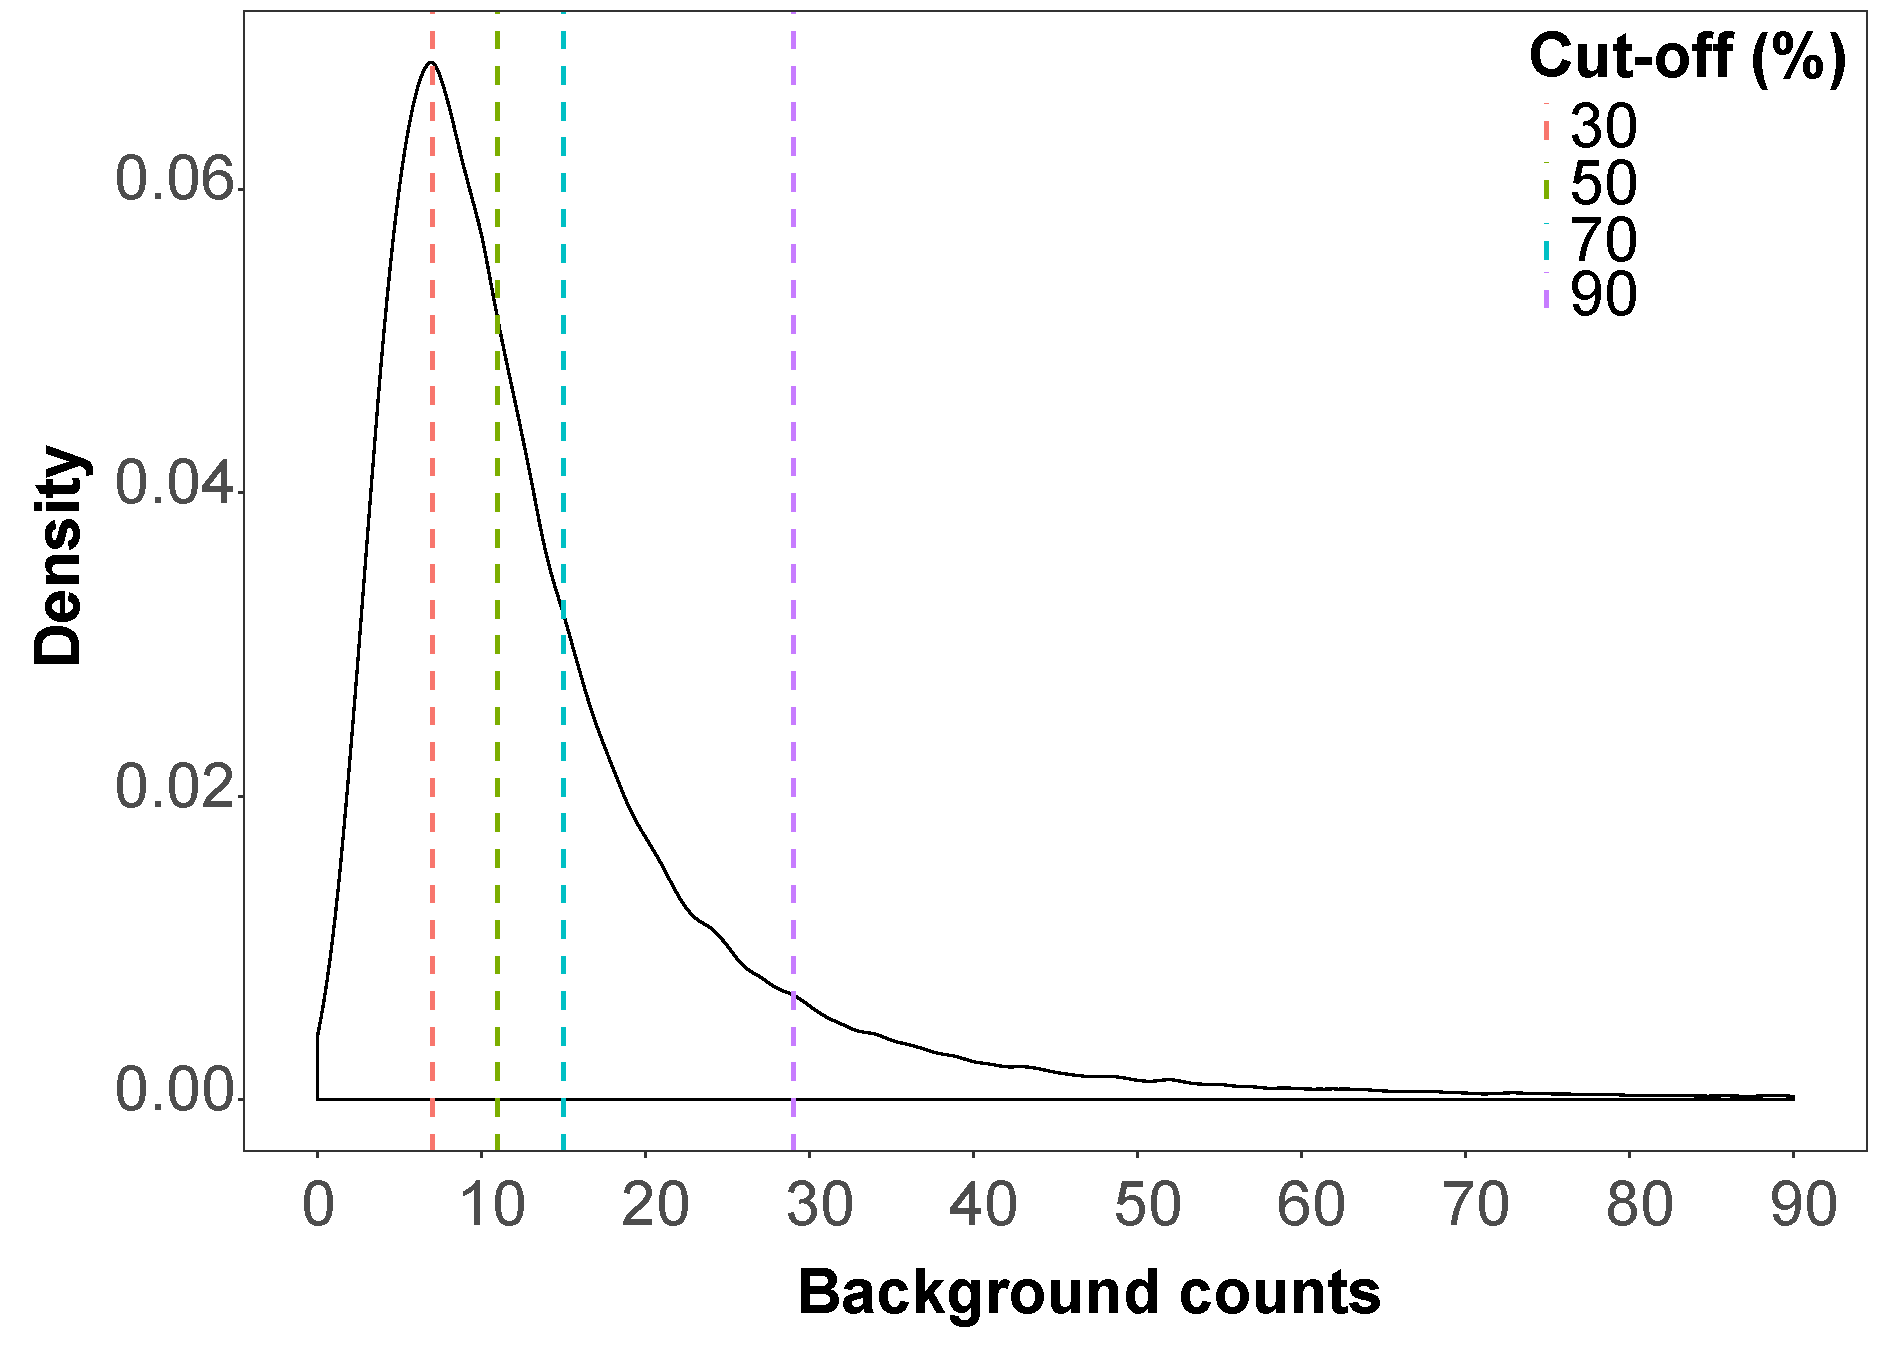
\includegraphics[width=0.5\textwidth]{./Appendix/pdfs/Chapter3/ATAC_absent_peaks_noise_distribution}
\caption[Distribution of the background read counts from all the master list peaks absent in each sample.]{\textbf{Distribution of the background read counts from all the master list peaks absent peaks in each sample.} Each cut-off corresponds to the number of background counts showed by a particular percentage of the total number of absent peaks.}
\label{figure:ATAC_absent_peaks_distribution}
\end{figure}

\begin{figure}[htbp]
\centering
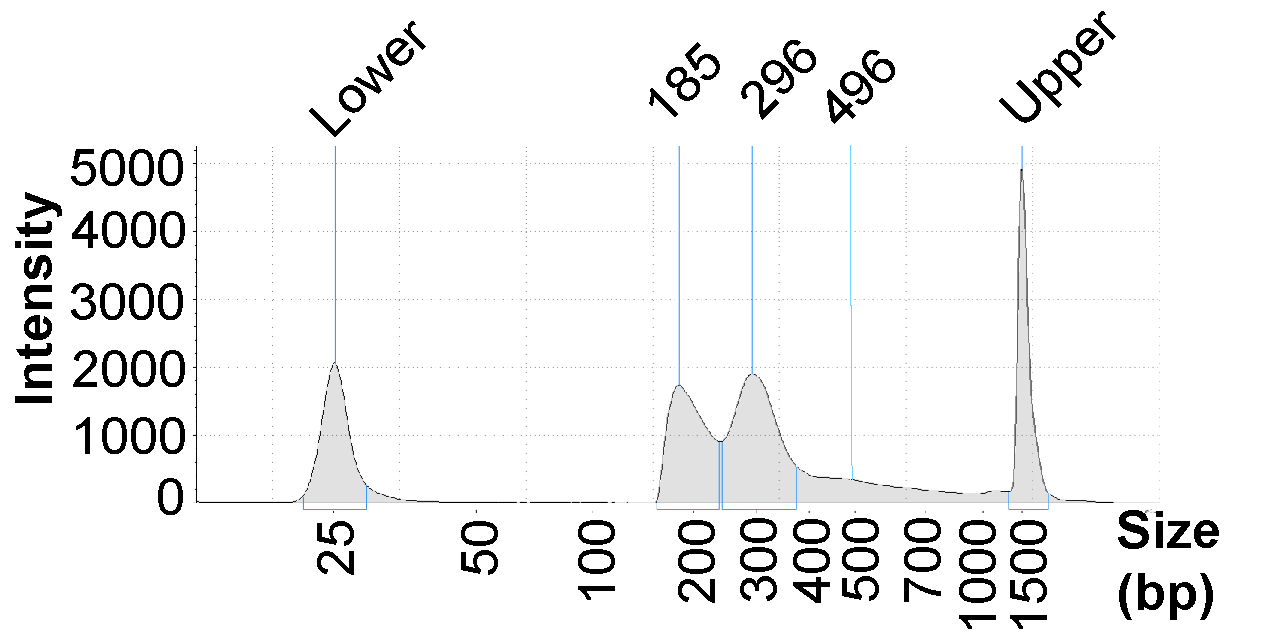
\includegraphics[width=0.5\textwidth]{./Appendix/pdfs/Chapter3/ATAC_PS02_tapestation_40min}
\caption[Pre-sequencing profiles of relative abundance of DNA library fragment sizes for a psoriatic lesional keratinocytes ATAC 1 library generated using 40 min of transposition.]{\textbf{Pre-sequencing profiles of relative abundance of DNA library fragment sizes for a psoriatic lesional keratinocytes ATAC 1 library generated using 40 min of transposition.} Pre-sequencing quantification of DNA fragment sizes from the ATAC library generated using 50,000 keratinocytes isolated from a psoriatic lesional skin biopsy and the ATAC 1 protocol (detailed in Table \ref{tab:ATAC_skin_optimisation_protocols}) and transposition for 40 min.}
\label{figure:PS2_40min_tapestation}
\end{figure}




\begin{figure}[htbp]
\centering
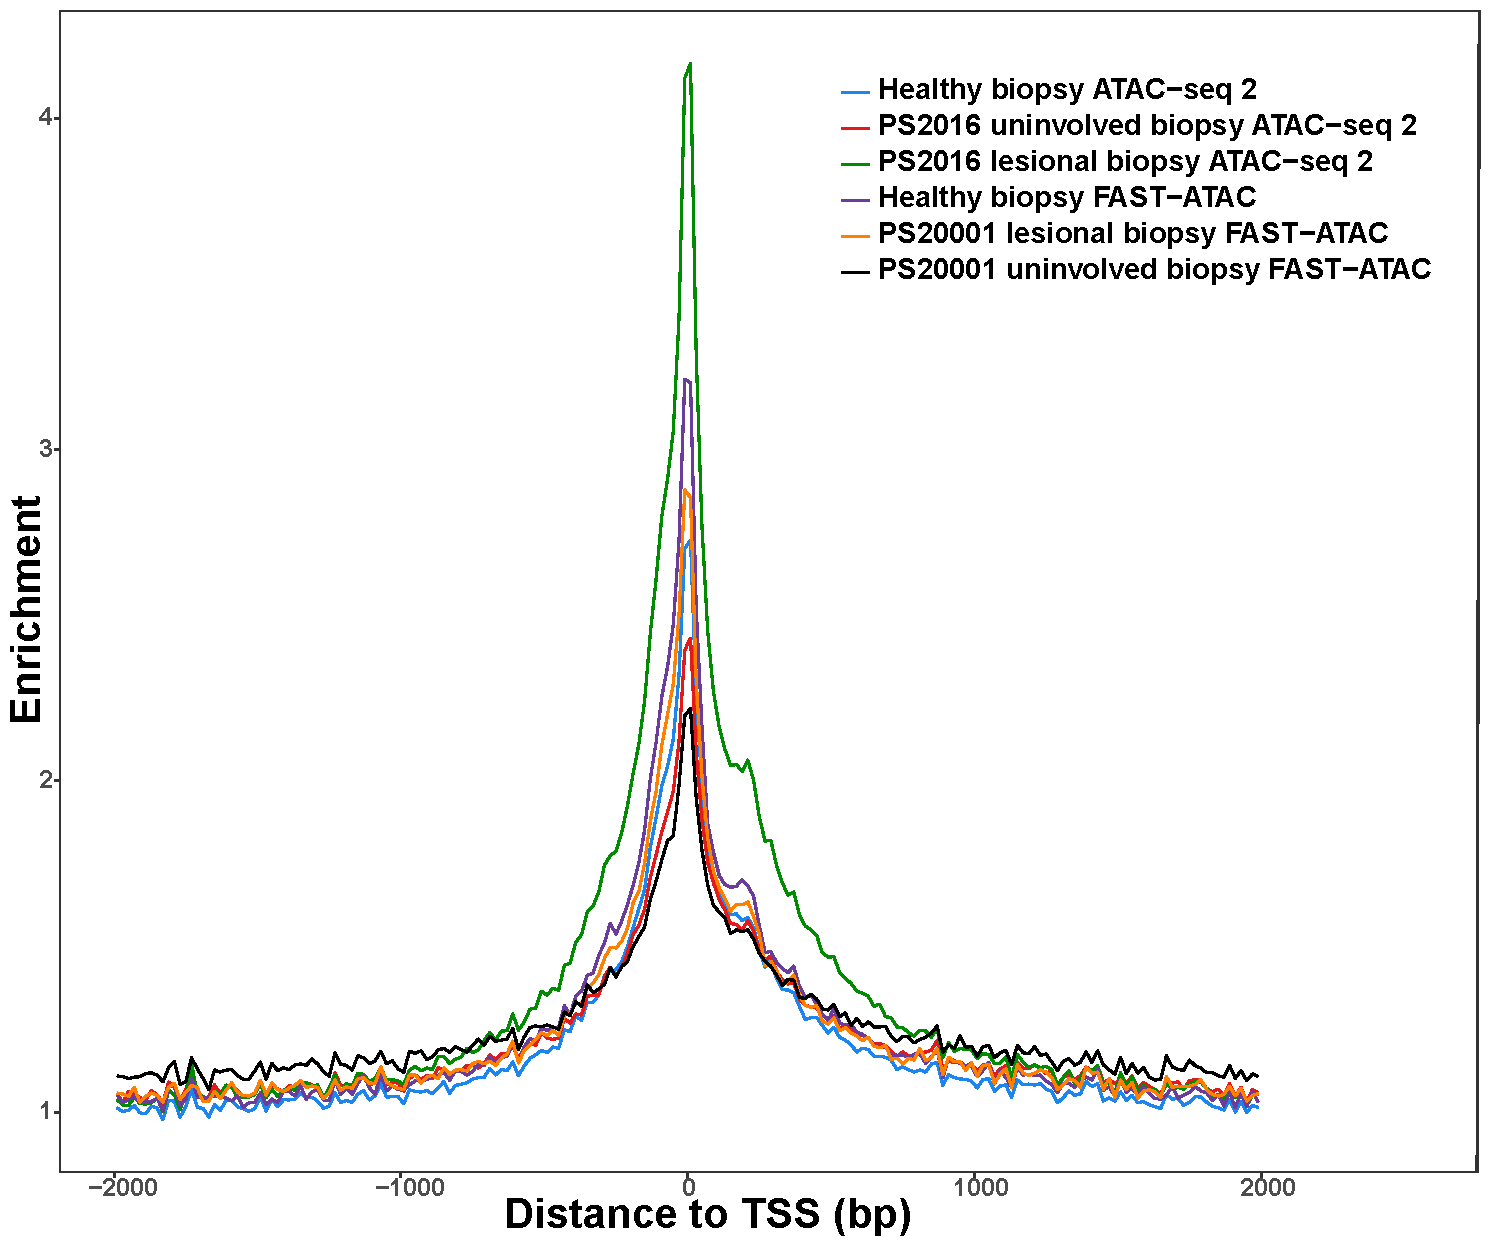
\includegraphics[width=0.5\textwidth]{./Appendix/pdfs/Chapter3/ATAC_skin_biopsy_samples_all_methods_TSS_enrichment_supplementary}
\caption[Assessment of TSS enrichment from ATAC 1 and Fast-ATAC in healthy and psoriasis KCs isolated from skin biopsy samples.]{\textbf{Assessment of TSS enrichment from ATAC 1 and Fast-ATAC in healthy and psoriasis KCs isolated from skin biopsy samples.} Fold-enrichment of ATAC fragments across the Ensembl annotated TSS from the different ATAC libraries.}
\label{figure:TSS_skin_biopsies}
\end{figure}



\begin{figure}[htbp]
\centering
\begin{subfigure}{0.70\textwidth}
\centering
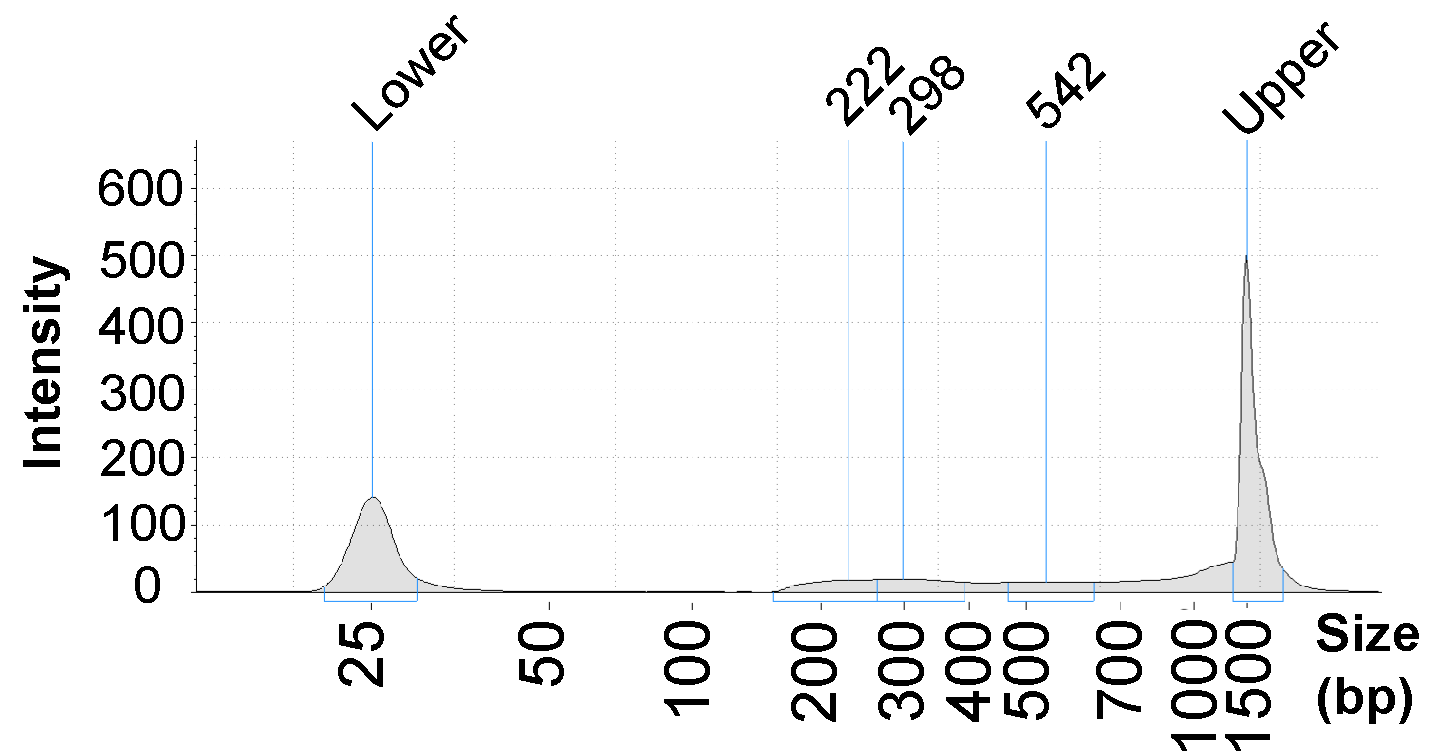
\includegraphics[width=\textwidth]{./Appendix/pdfs/Chapter3/FAST_ATAC_skin_tapestation_C1}
\caption{\textbf{}}
% The percentage sign indicated that the other subfig goes side by side
\end{subfigure}
\begin{subfigure}{0.60\textwidth}
\centering
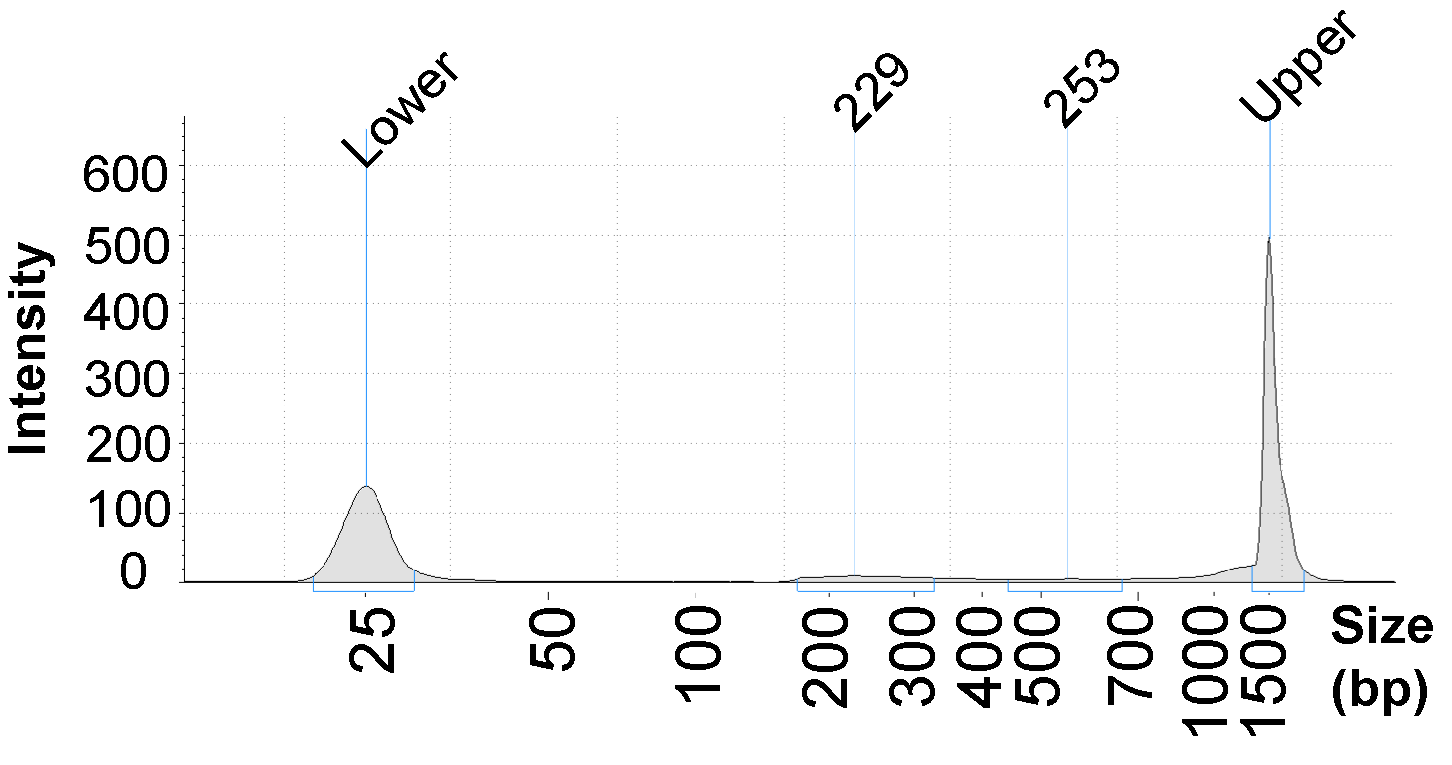
\includegraphics[width=\textwidth]{./Appendix/pdfs/Chapter3/FAST_ATAC_skin_tapestation_C3}
\caption{\textbf{}}
\end{subfigure}
\begin{subfigure}{0.60\textwidth}
\centering
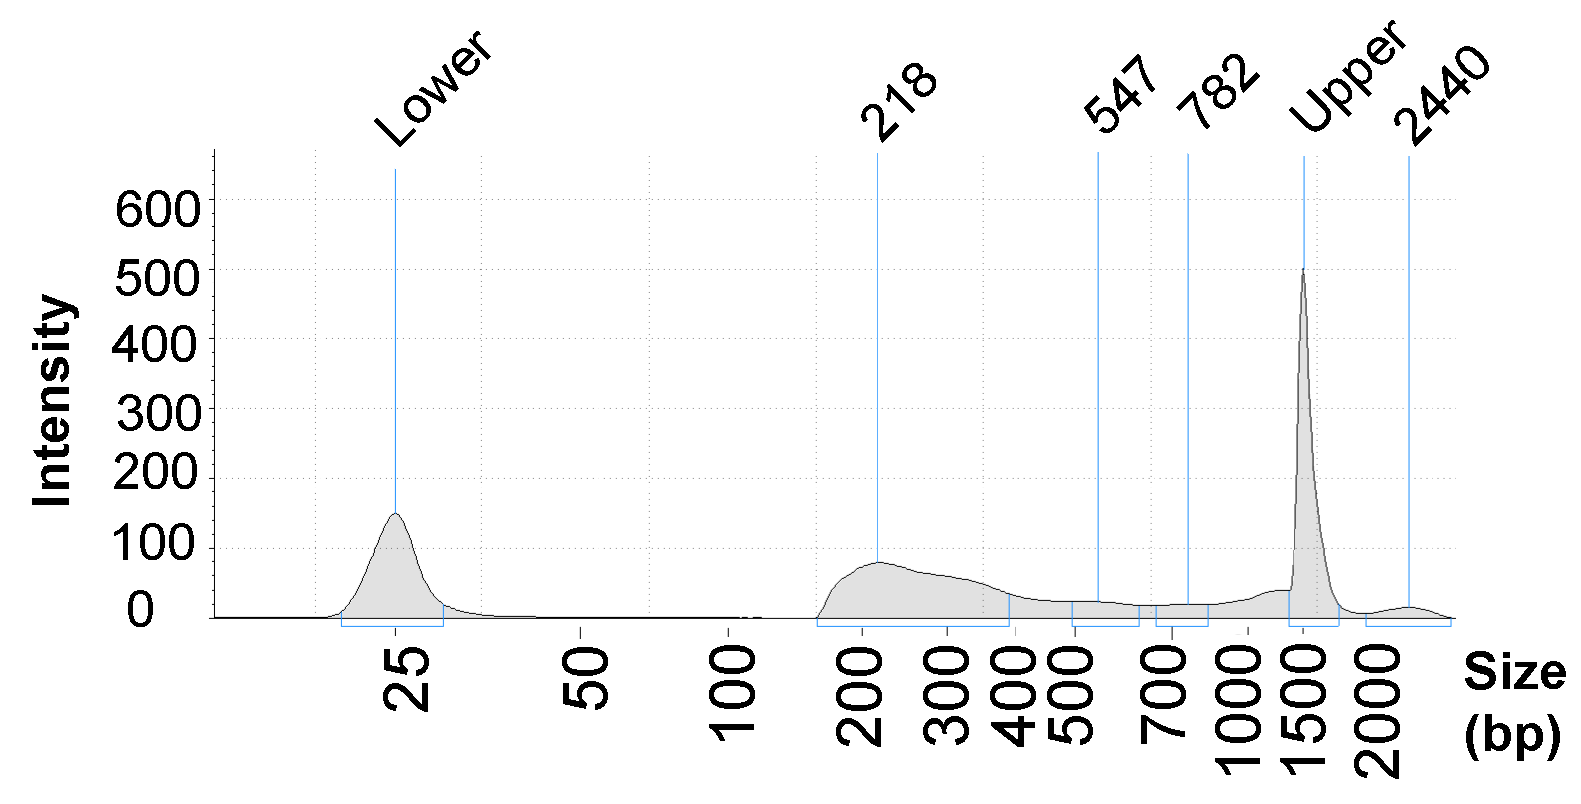
\includegraphics[width=\textwidth]{./Appendix/pdfs/Chapter3/FAST_ATAC_skin_tapestation_C4}
\caption{\textbf{}} % to add text to the figure name
\end{subfigure}
\begin{subfigure}{0.60\textwidth}
\centering
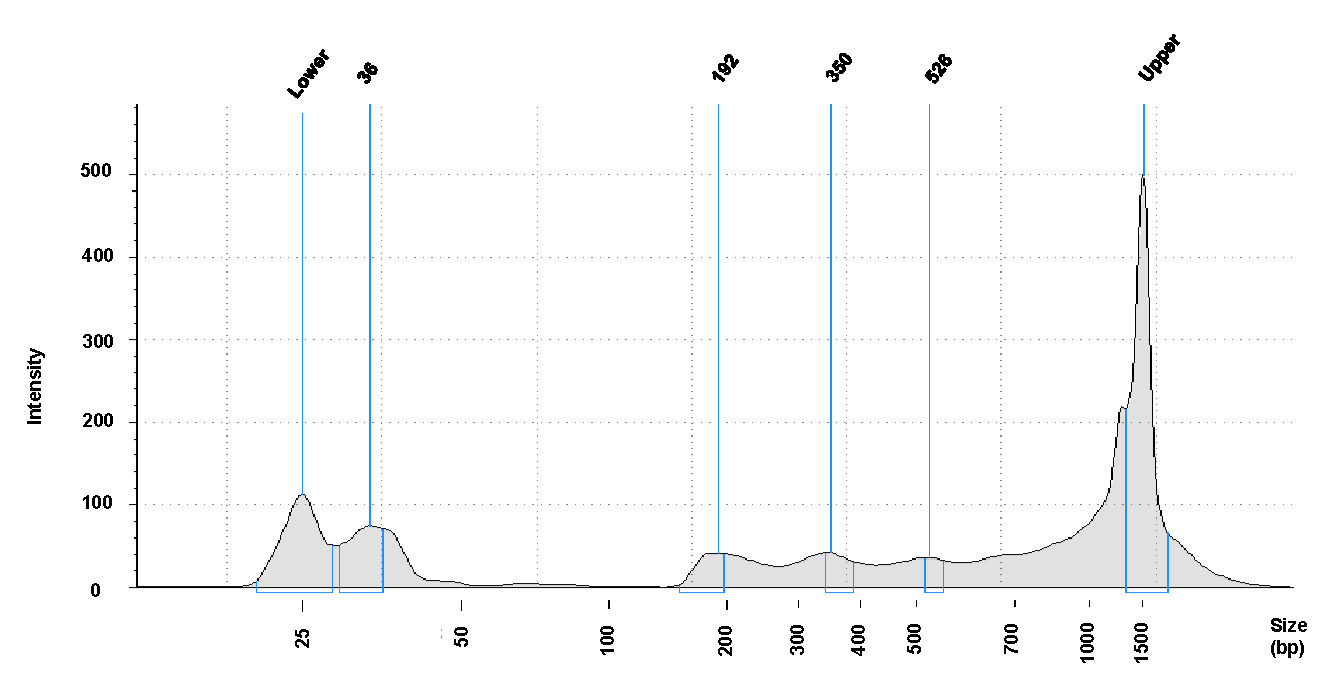
\includegraphics[width=\textwidth]{./Appendix/pdfs/Chapter3/Omni_ATAC_NHEK_Rep1_tapestation}
\caption{\textbf{}} % to add text to the figure name
\end{subfigure}
\hfill
\caption[Fast-ATAC and Omni-ATAC NHEK pre-sequencing profiles of relative abundance of DNA library fragment sizes.]{\textbf{Fast-ATAC and Omni-ATAC NHEK pre-sequencing profiles of relative abundance of DNA library fragment sizes.} Pre-sequencing quantification of DNA fragment sizes from the libraries generated  using the (A) C2, (B) C3, and (C) C4 versions of the Fast-ATAC protocol based on modifications in the detergent and Tn5 concentration and (D) Omni-ATAC. C2, C3 and C4 detergent and Tn5 concentrations are detailed in Table \ref{tab:ATAC_skin_optimisation_protocols}.}
\label{figure:NHEK_tapestation}
\end{figure}


\clearpage


\section{Chapter 4 Figures}

\begin{figure}[htbp]
\centering
\begin{subfigure}{0.45\textwidth}
\centering
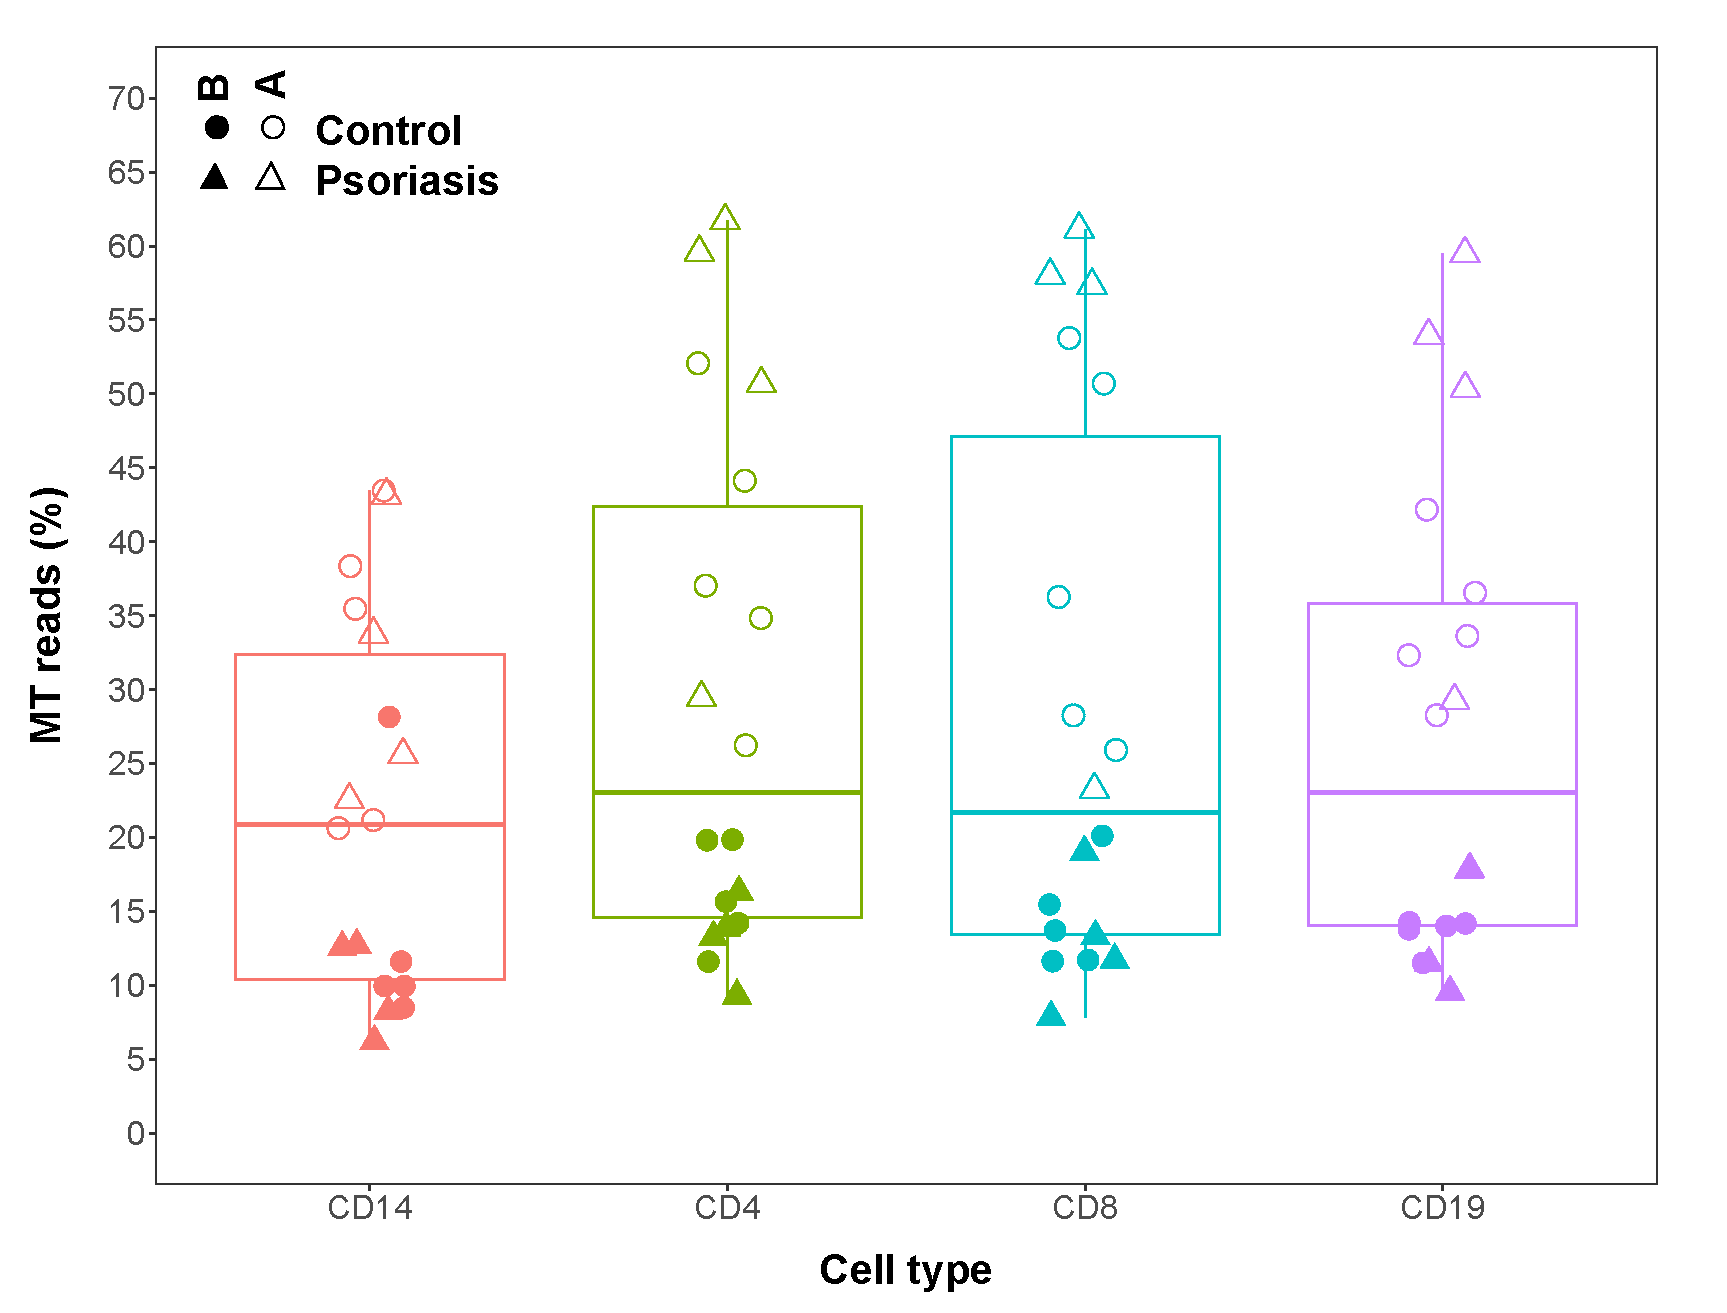
\includegraphics[width=\textwidth]{./Appendix/pdfs/Chapter4/ATAC_PS_CTL_MT_percent_boxplot}
\caption{\textbf{}}
\end{subfigure}
\begin{subfigure}{0.5\textwidth}
\centering
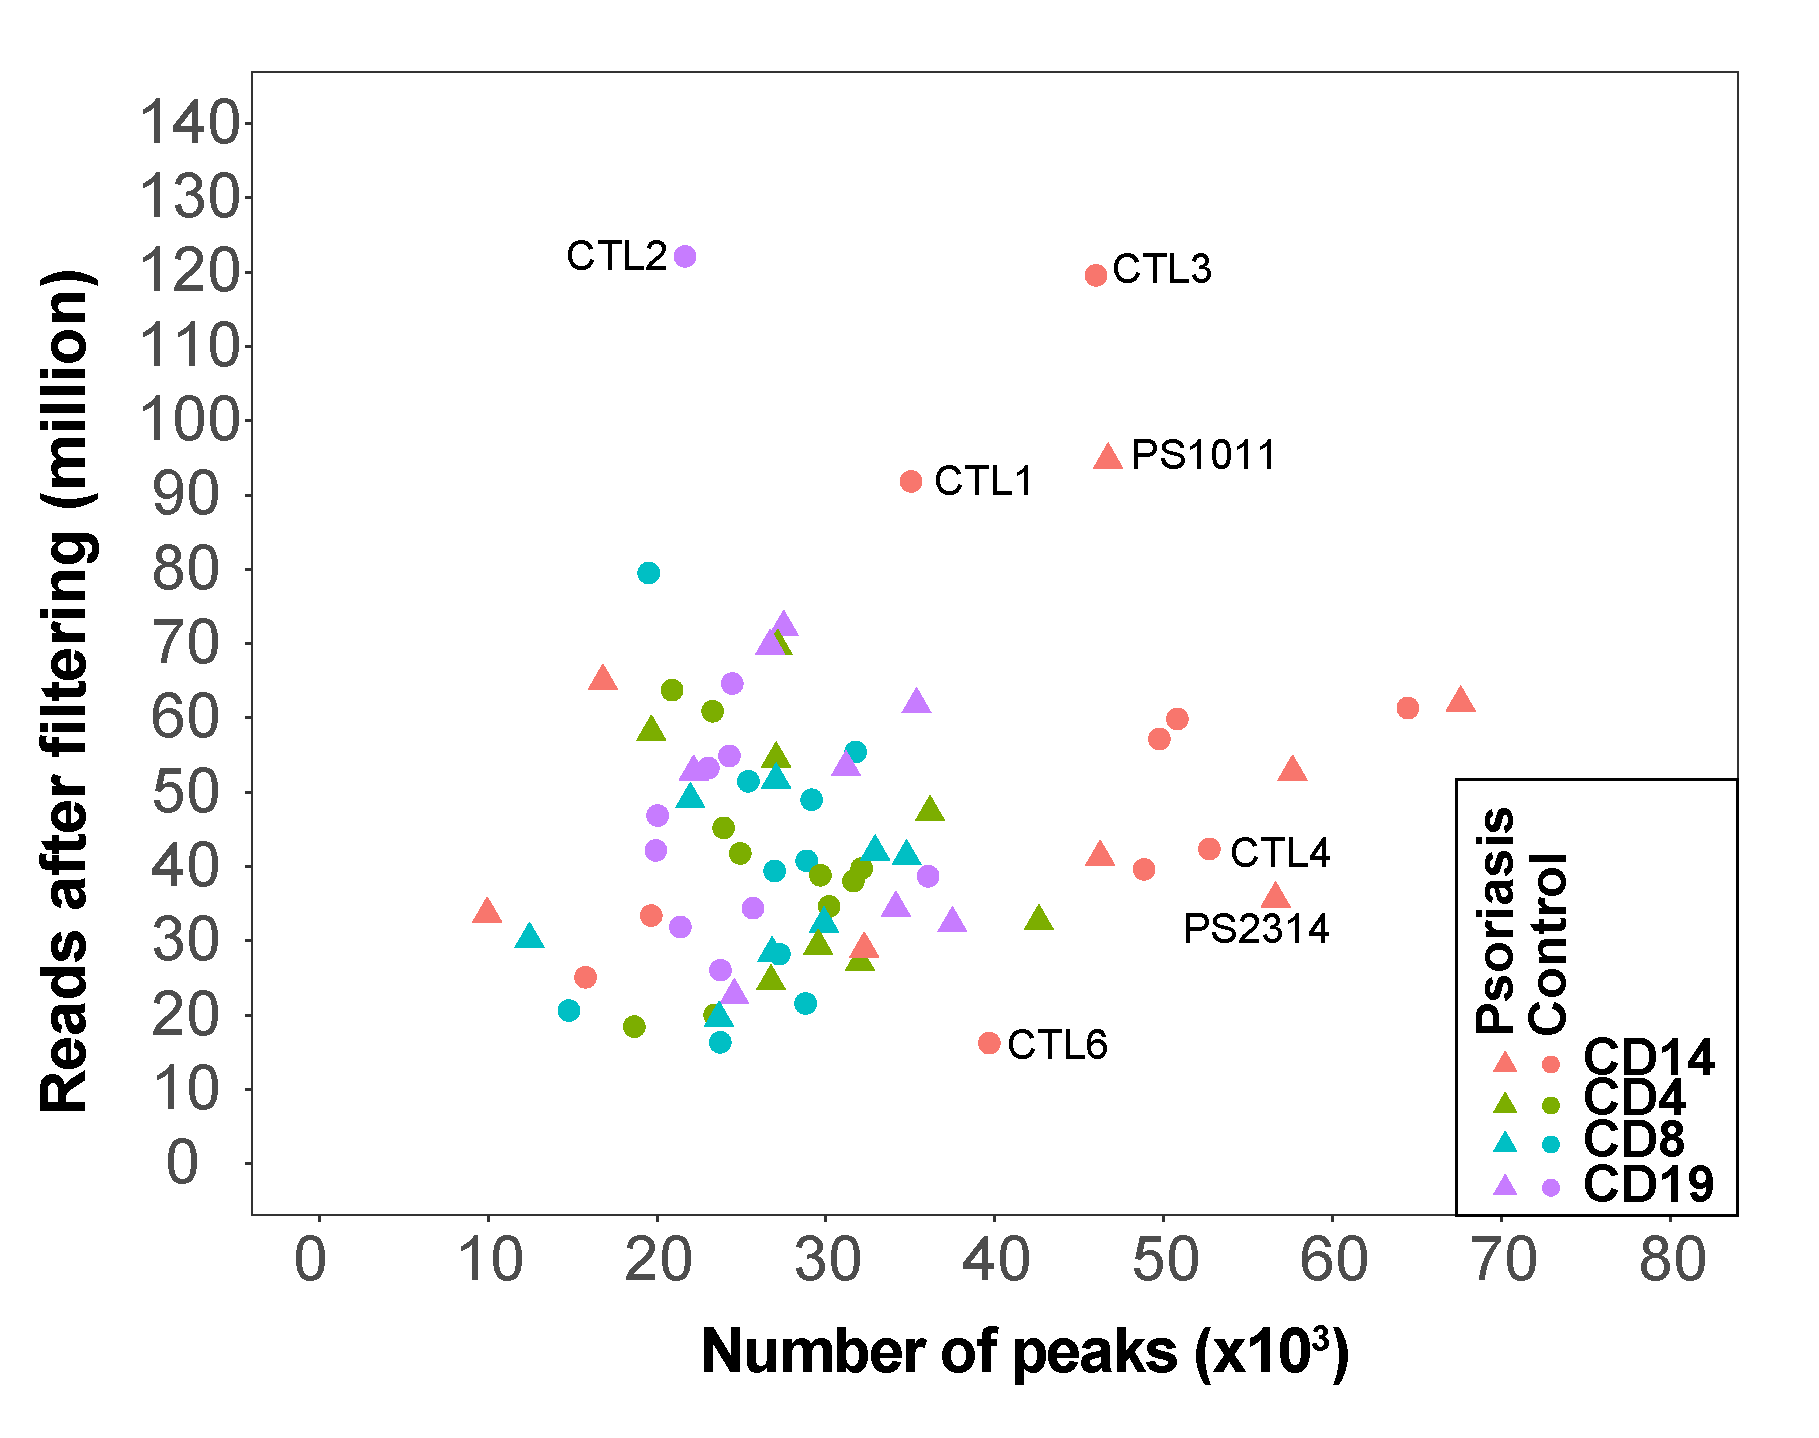
\includegraphics[width=\textwidth]{./Appendix/pdfs/Chapter4/ATAC_PS_CTL_reads_vs_peaks_dotplot}
\caption{\textbf{}}
\end{subfigure}
\caption[Percentage of MT reads and called peaks after IDR p-value filtering in the ATAClibraries generated in CD14$^+$ monocytes, CD4$^+$, CD8$^+$ and CD19$^+$ isolated from psoriasis patients and healthy controls.]{\textbf{(A) Percentage of MT reads in the ATAC-seq samples generated in CD14$^+$ monocytes, CD4$^+$, CD8$^+$ and CD19$^+$ isolated from psoriasis patients and healthy controls.} Samples from cohort 1A (open circlues and triangles) were generated with the standard ATAC-seq protocol from Buenrostro \textit{et al.}, 2013 whereas samples from cohort 1B (filles circles and triangles) were processed using FAST-ATAC \parencite{Corces2016}. (B) For each of the ATAC libraries, representation of the number of significant peaks based on IDR optimal p-value filtering versus the total million of reads after filtering.}
\label{figure:ATAC_PS_CTL_MT_percent_and_called_peaks}
\end{figure}


%\begin{figure}[htbp]
%\centering
%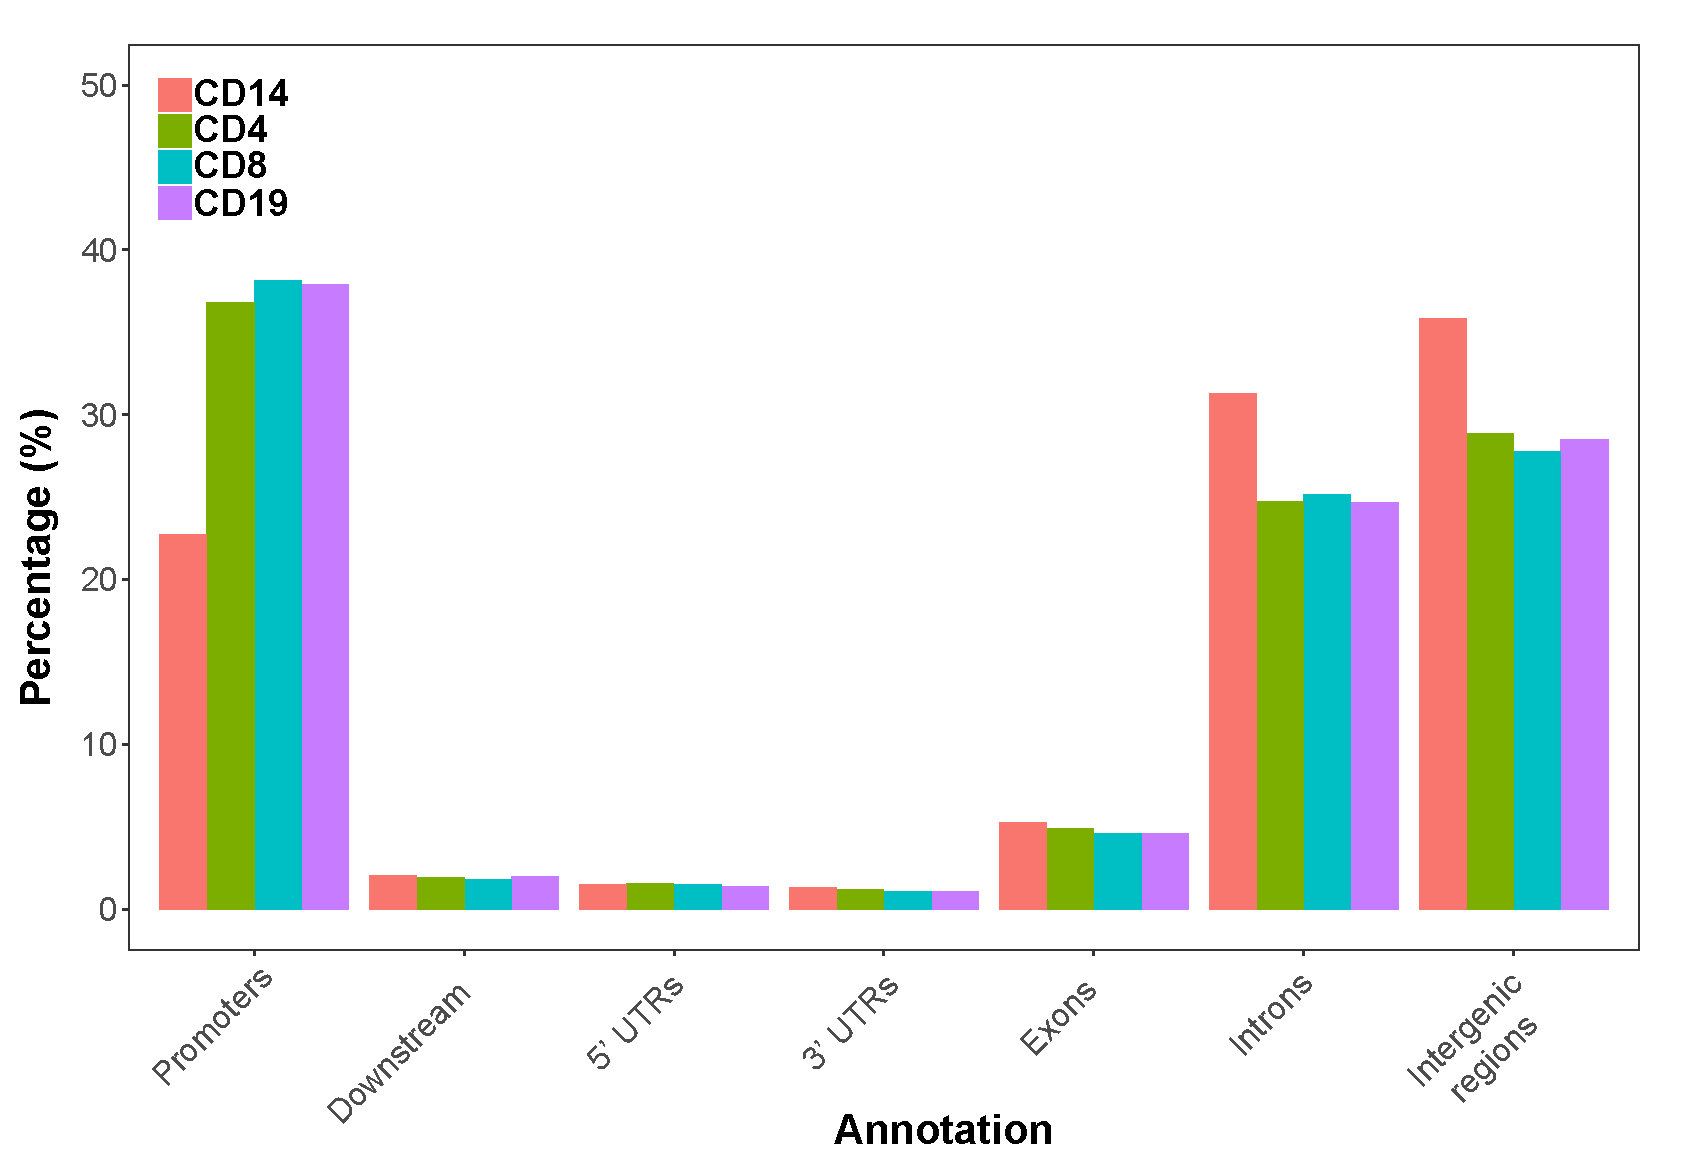
\includegraphics[width=0.6\textwidth]{./Appendix/pdfs/Chapter4/ATAC_all_cell_types_individual_master_lists_general_peak_annotation}
%\caption[Genomic annotation of the consensus master list of ATAC-seq enriched sites built for downstream differential chromatin accessibility analysis in CD14$^+$ monocytes, CD4$^+$, CD8$^+$ and CD19$^+$.]{\textbf{Genomic annotation of the consensus master list of ATAC-seq enriched sites built for downstream differential chromatin accessibility analysis in CD14$^+$ monocytes, CD4$^+$, CD8$^+$ and CD19$^+$.} Annotation is expressed in percentage over the total number of ATAC-seq sites included in each particular cell type master list.}
%\label{fig:ATAC_PS_CTL_genomic_annotation}
%\end{figure}


\bigskip
\begin{figure}[htbp]
\centering
\begin{subfigure}[b]{0.50\textwidth}
\centering 
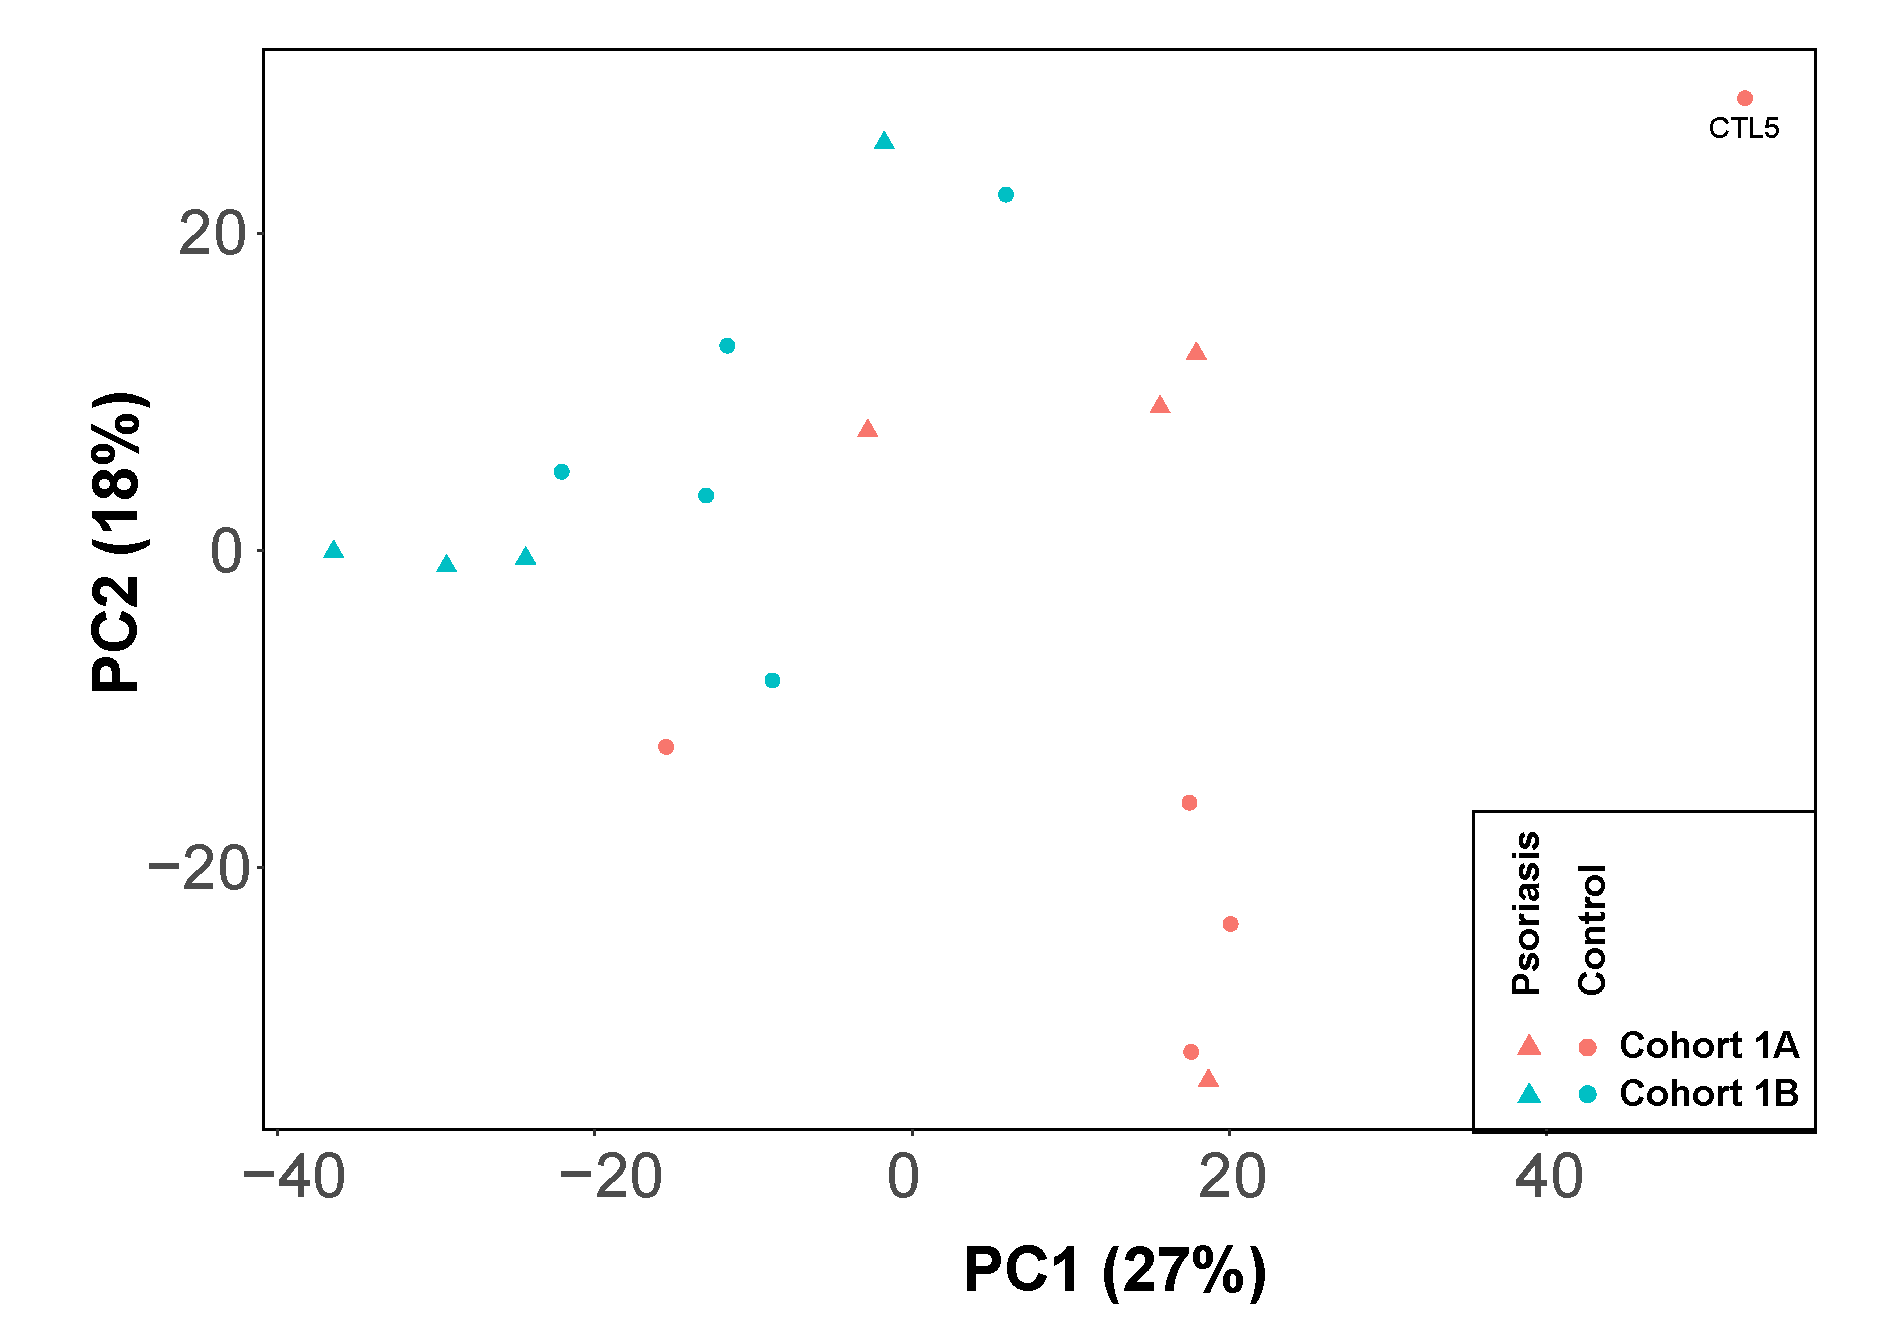
\includegraphics[width=\textwidth]{./Appendix/pdfs/Chapter4/ATAC_CD8_PS_CTL_PCA}
\caption{}
\end{subfigure}
~
\begin{subfigure}[b]{0.50\textwidth} 
%the [b] prevents offset in subcaptions
\centering
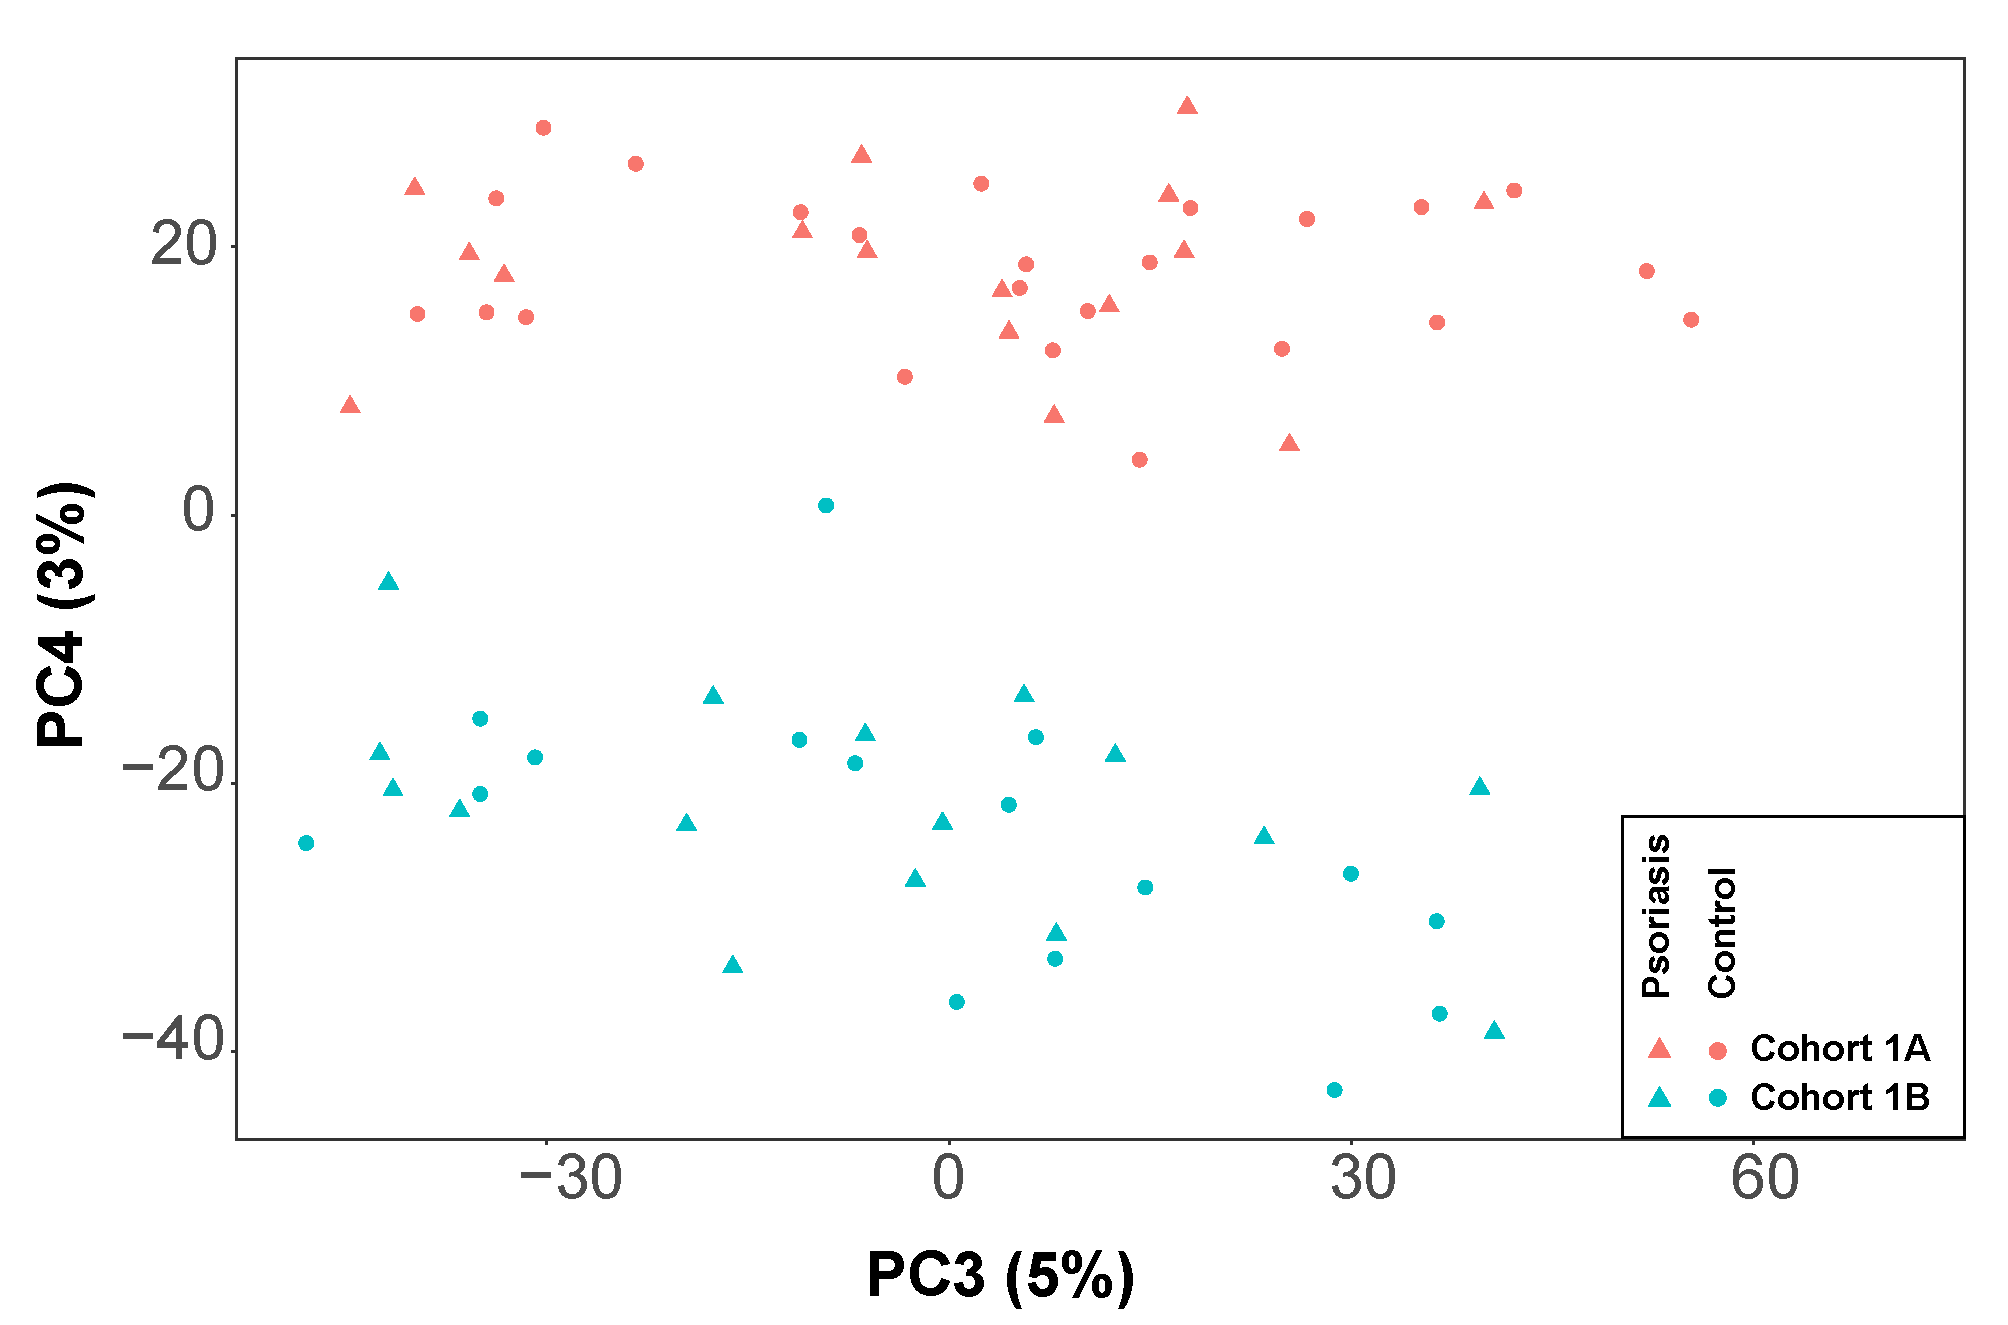
\includegraphics[width=\textwidth]{./Appendix/pdfs/Chapter4/PS_CTL_all_samples_varied_PCA3and4_plot}
\caption{}
\end{subfigure}
\caption[PCA analysis illustrating batch effect in ATAC and RNA-seq samples.]{\textbf{PCA analysis illustrating batch effect in ATAC and RNA-seq samples.} (A) First and second component of the PCA analysis performed using the normalised ATAC  counts in a master list of consensus regions across all the combined tCD8$^+$ samples from psoriasis patients and healthy controls. b) Third and fourth component of the PCA analysis performed on the normalised number of reads mapping to the Ensmbl list of mRNAs and lncRNAs detected in tCD8$^+$ cells from psoriasis patients and healthy controls. For each dot colour corresponds to cohort ID (batch) and shape to condition (psoriasis or control).}
\label{figure:ATAC_RNAseq_batch_effect}
\end{figure}



\begin{figure}[htbp]
\centering
\begin{subfigure}{0.5\textwidth}
\centering
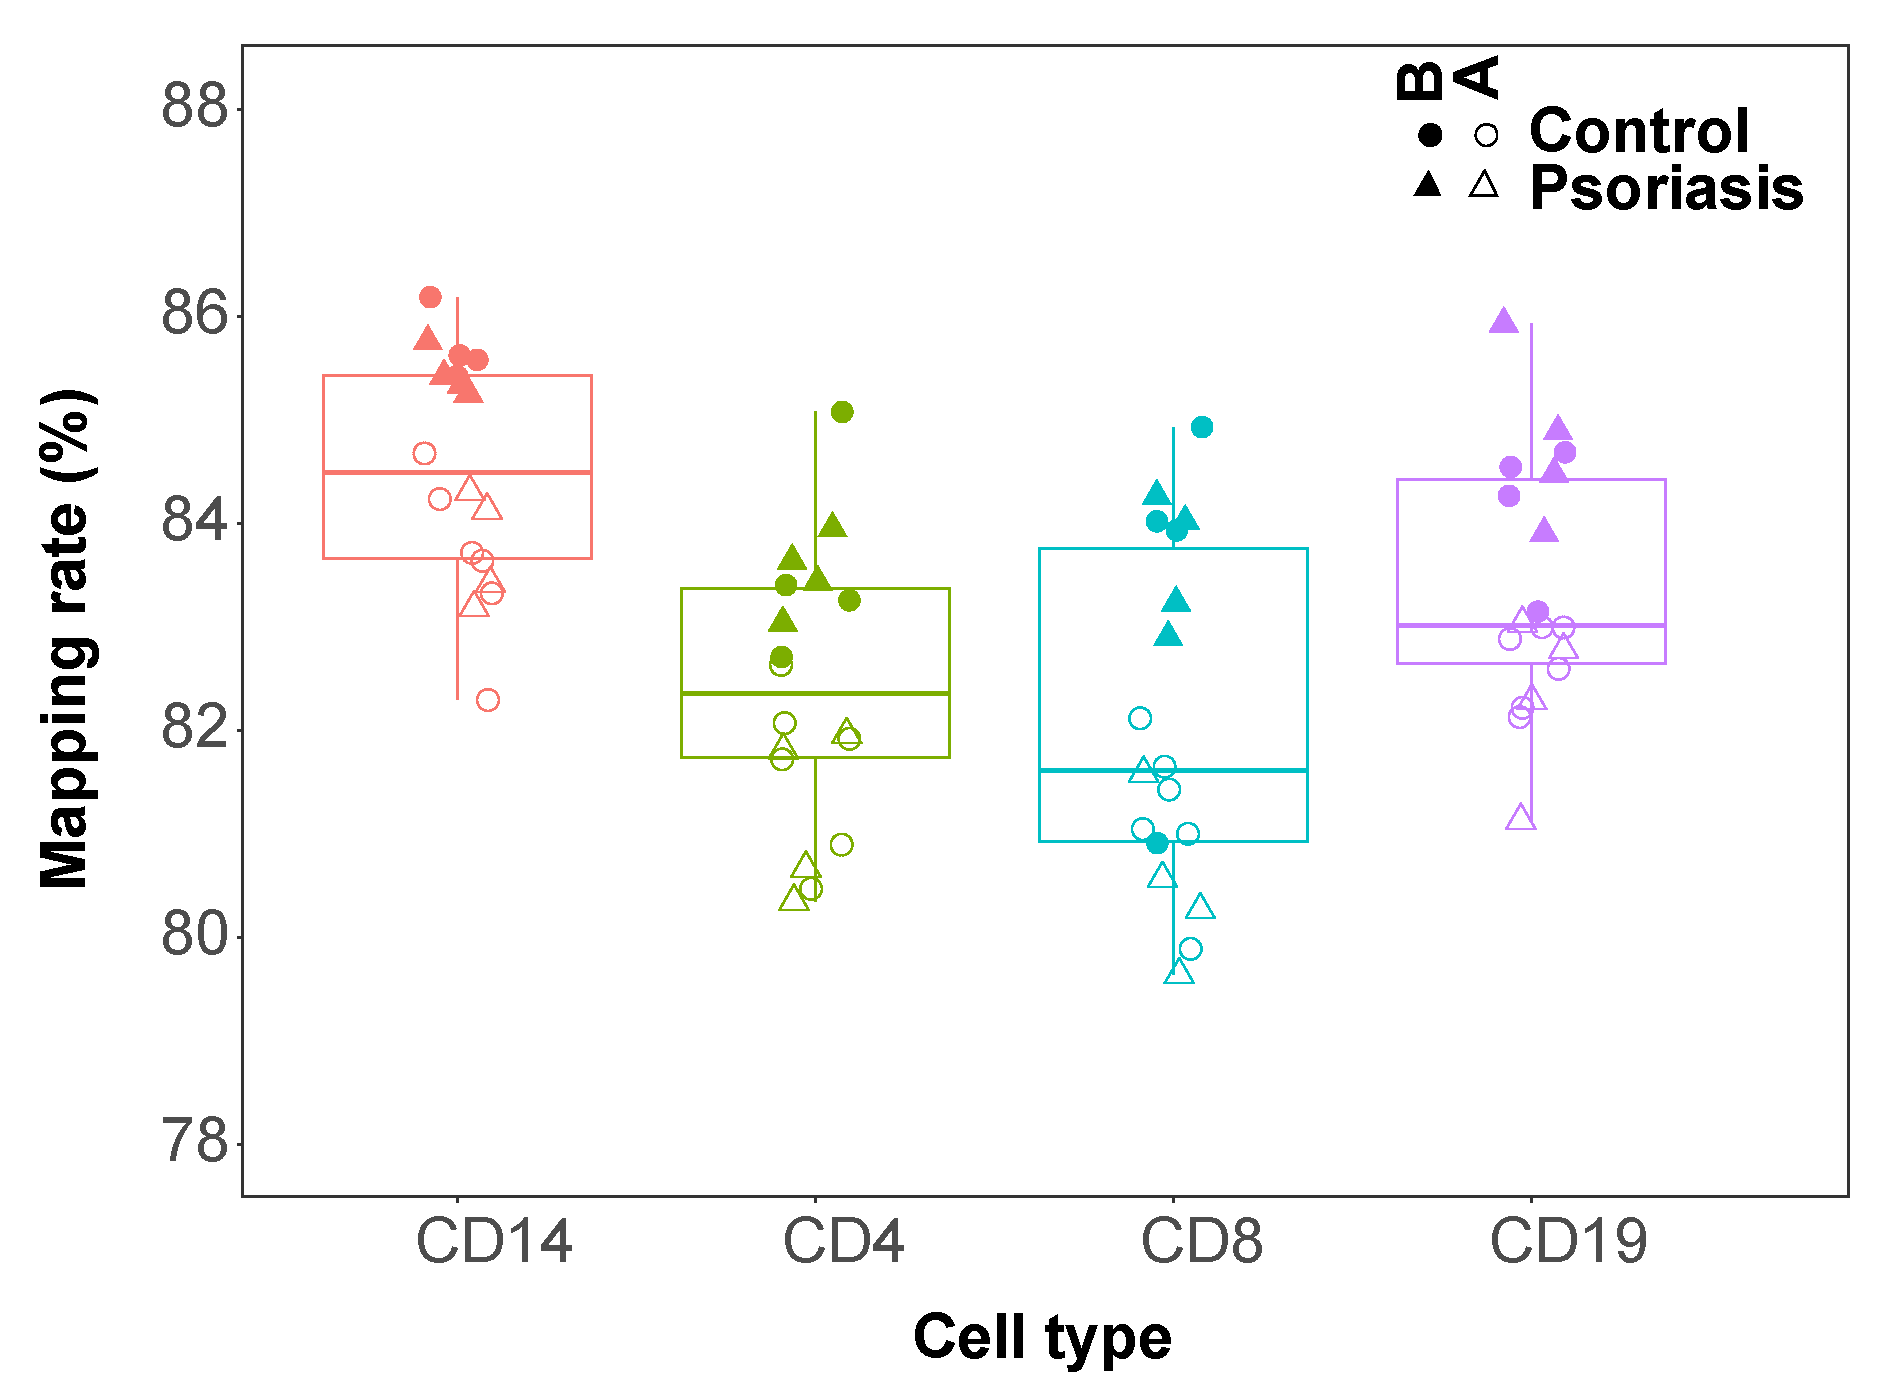
\includegraphics[width=\textwidth]{./Appendix/pdfs/Chapter4/PS_CTL_RNAseq_uniquely_mapped_reads_rate_cell_type_batch_and_condition_boxplots}
\caption{\textbf{}}
% The percentage sign indicated that the other subfig goes side by side
\end{subfigure}%
\begin{subfigure}{0.5\textwidth}
\centering
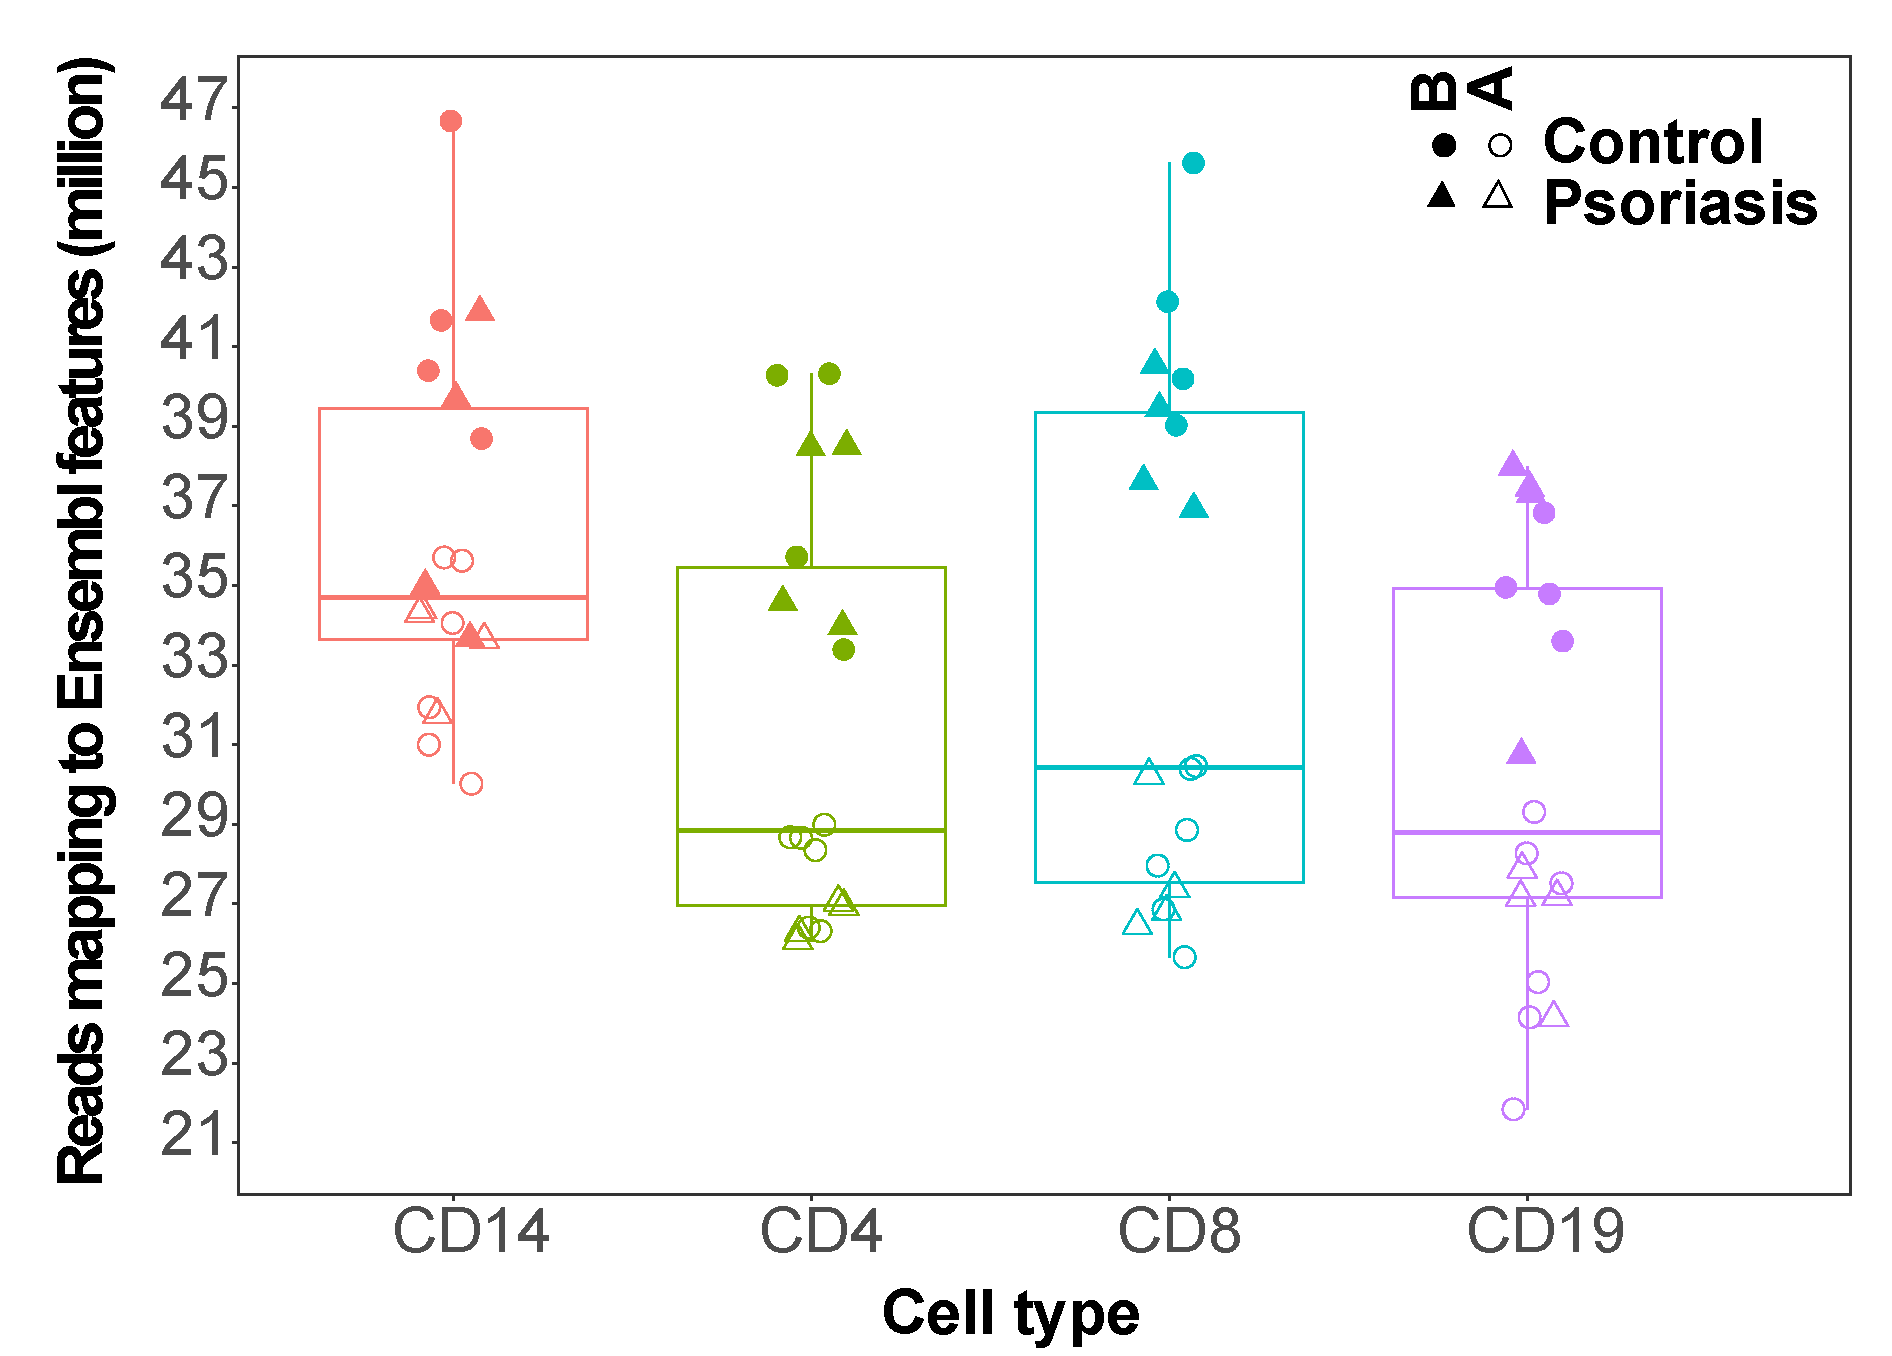
\includegraphics[width=\textwidth]{./Appendix/pdfs/Chapter4/PS_CTL_RNAseq_total_reads_per_batch_cell_type_and_condition}
\caption{\textbf{}}
\end{subfigure}
\caption[Mapping rate and total reads after filtering (million) mapping to Ensembl genes in all the RNA-seq samples from psoriasis patients and controls in four cell types.]{\textbf{Mapping rate and total reads after filtering (million) mapping to Ensembl genes in all the RNA-seq samples from psoriasis patients and controls in four cell types.} (A) The mapping rate refers to the percentage of total sequenced reads from each sample that uniquely mapped to a particular site of the genome. (B) The total number of reads after filtering for non-uniquely mapped and duplicated reads that mapped to Ensembl features, including coding protein genes and lncRNAs.}
\label{figure:RNAseq_mapping_rate_and_reads_in_genes}
\end{figure} 


\begin{figure}[htbp]
\centering
\begin{subfigure}{0.45\textwidth}
\centering
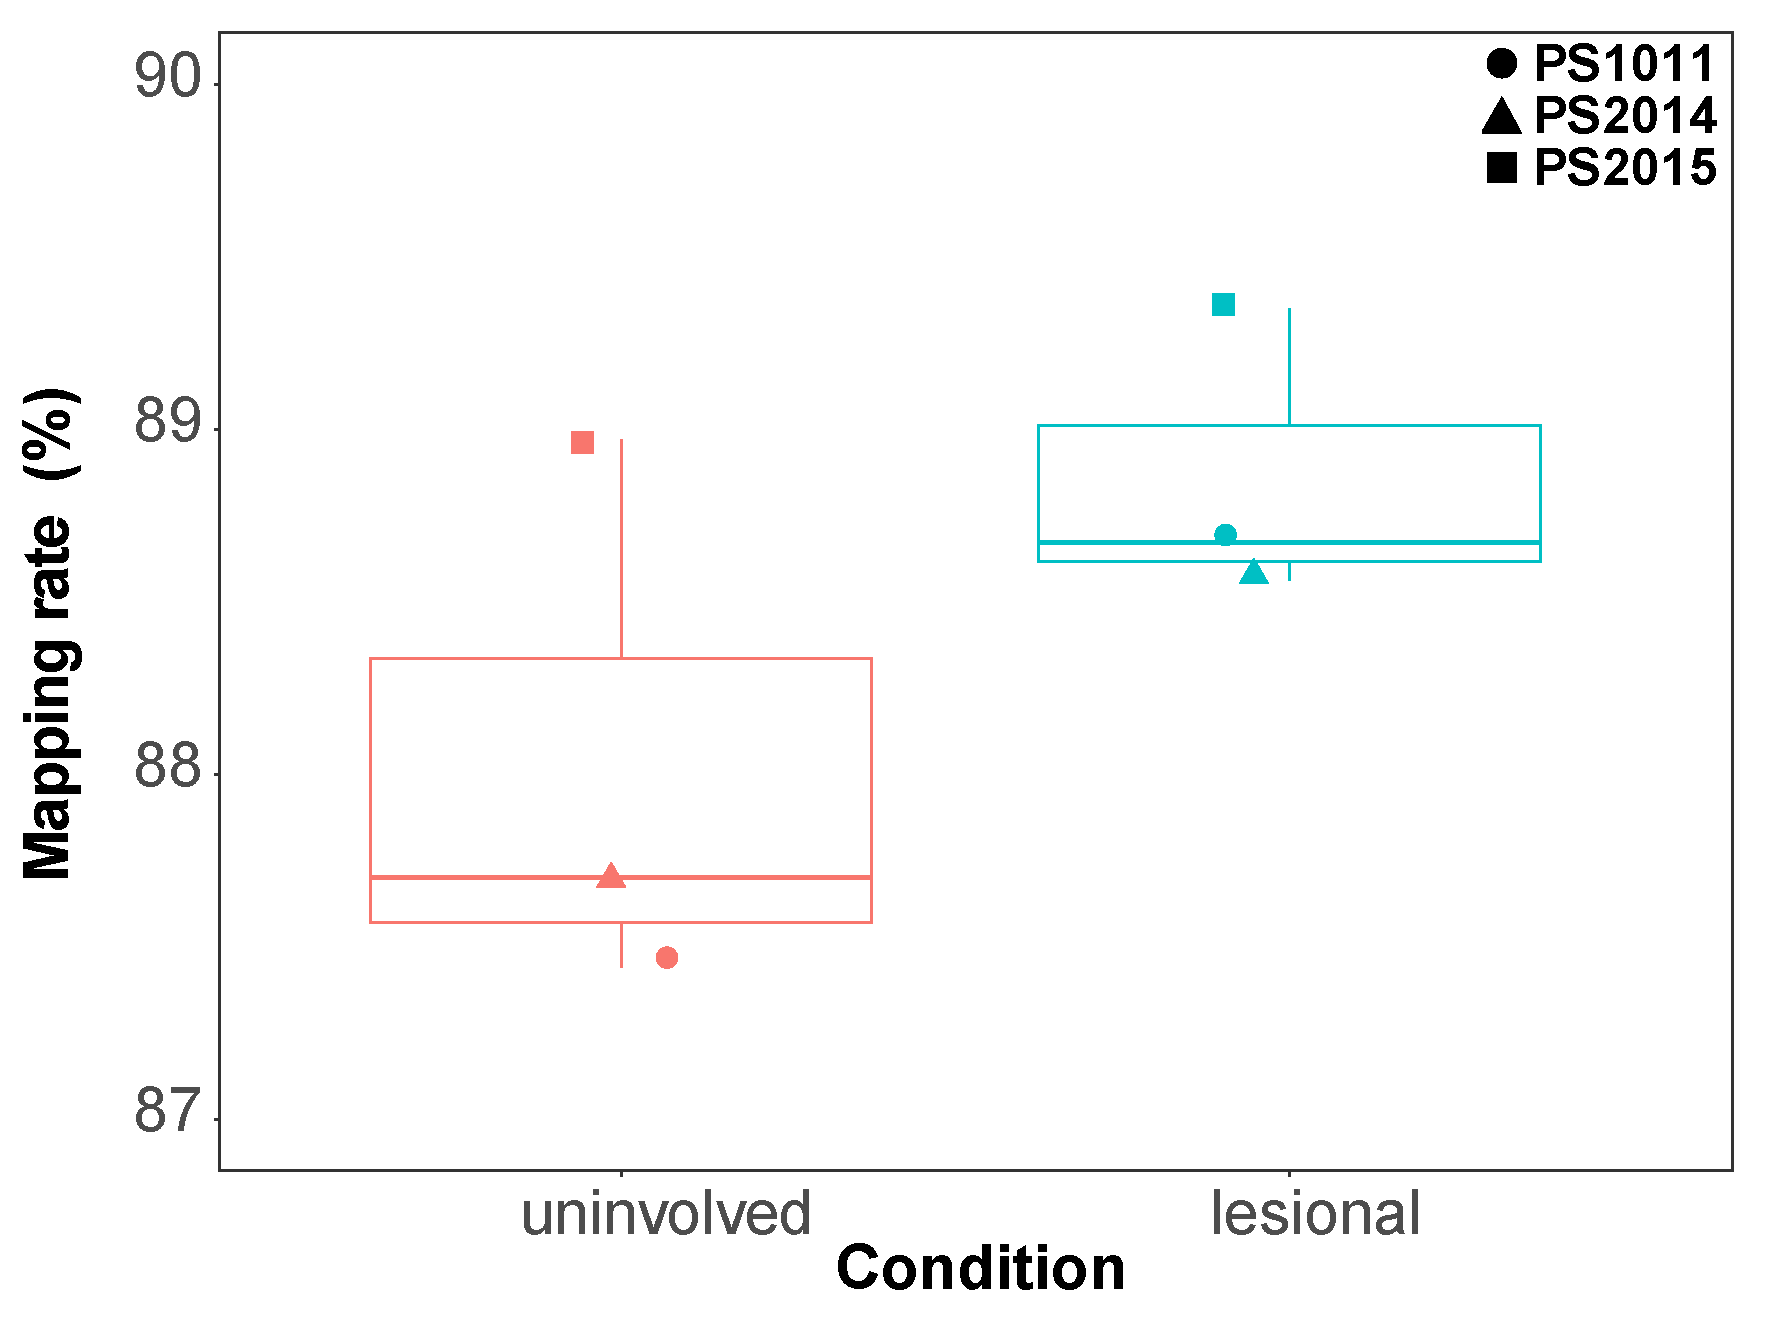
\includegraphics[width=\textwidth]{./Appendix/pdfs/Chapter4/PS_lesional_uninvolved_RNAseq_uniquely_mapped_reads_percent_cell_type_and_batch_boxplots}
\caption{\textbf{}}
% The percentage sign indicated that the other subfig goes side by side
\end{subfigure}%
\begin{subfigure}{0.45\textwidth}
\centering
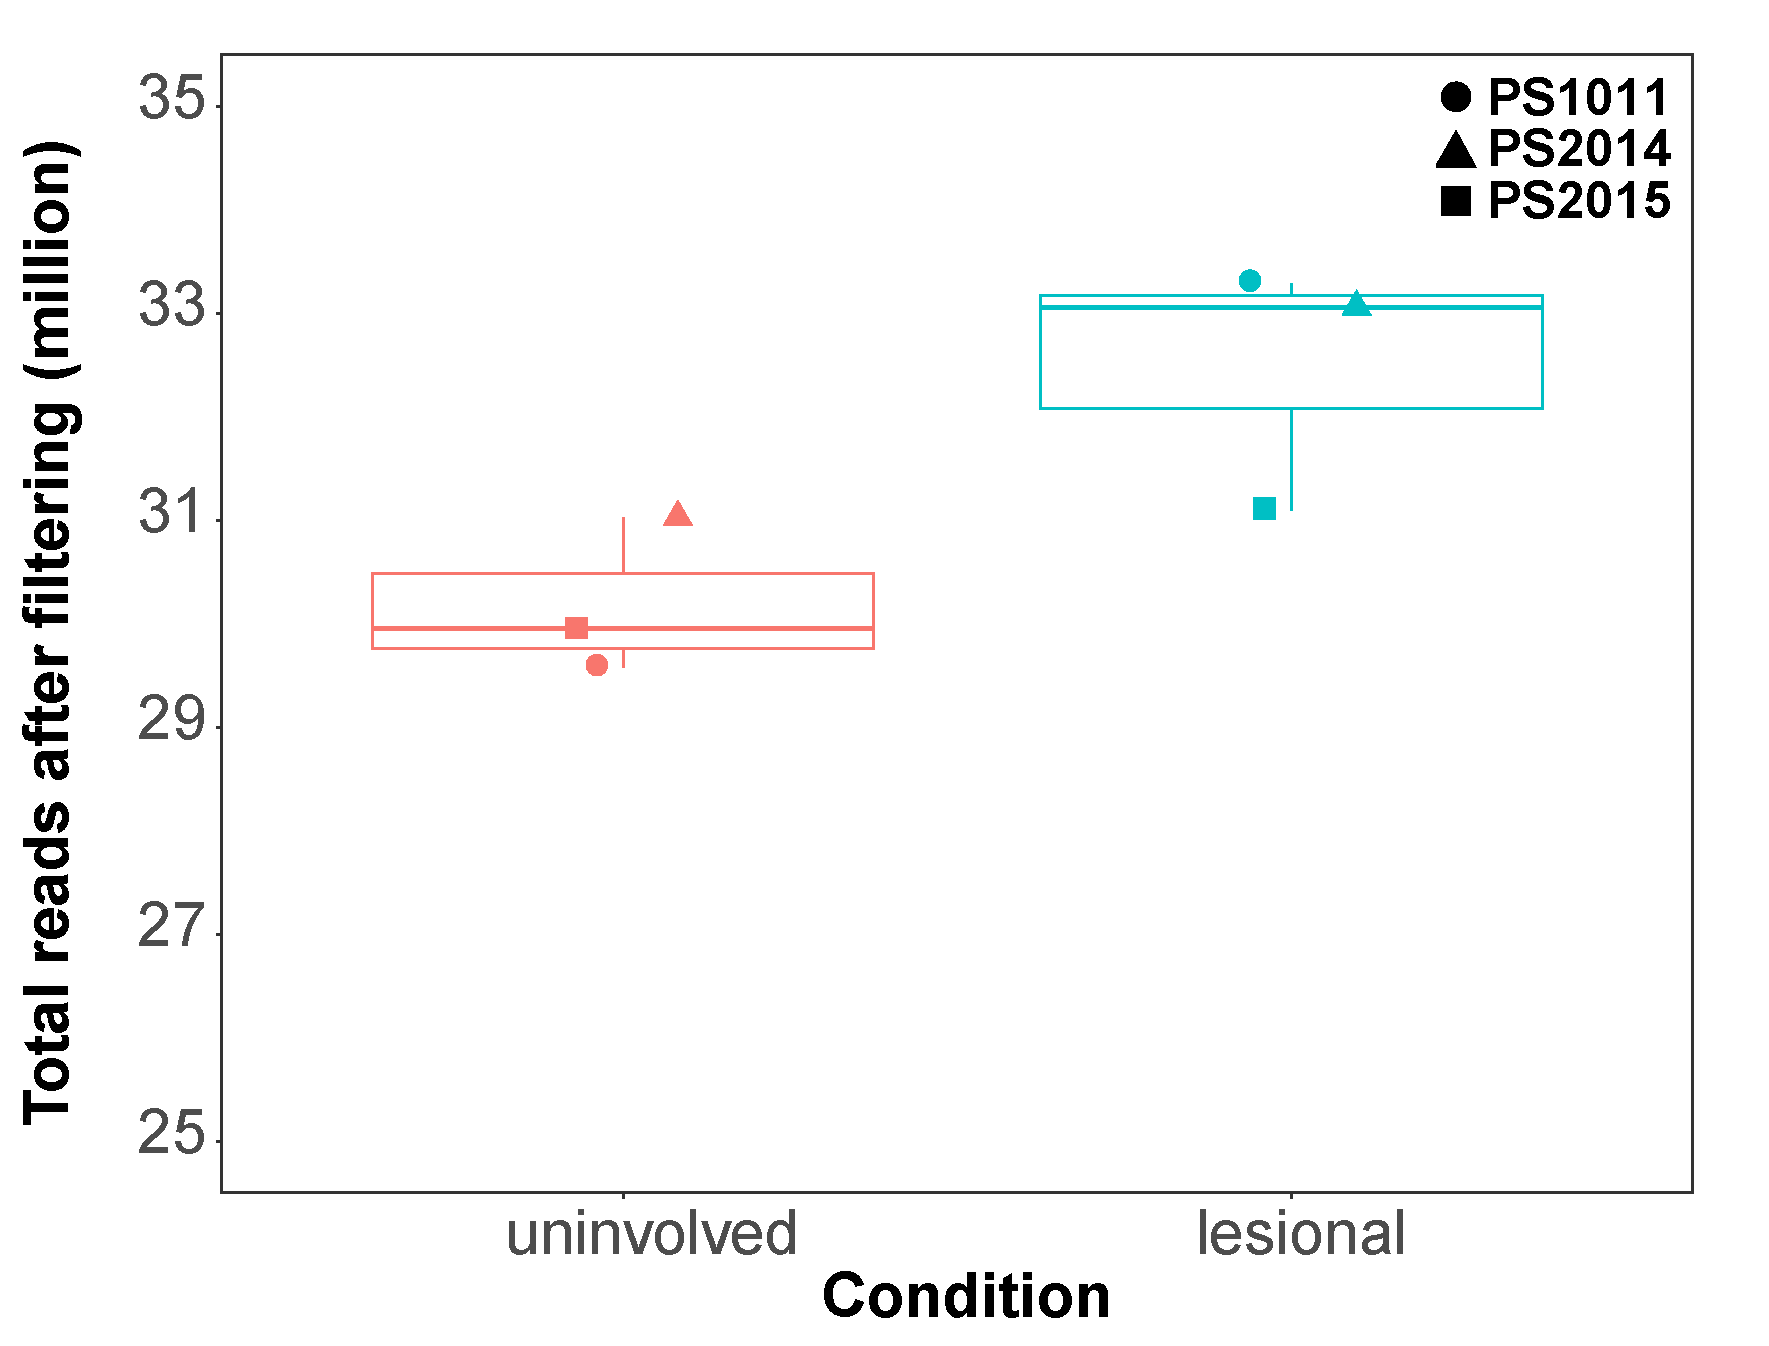
\includegraphics[width=\textwidth]{./Appendix/pdfs/Chapter4/PS_lesional_uninvolved_RNAseq_total_reads_per_cell_type_and_batch}
\caption{\textbf{}}
\end{subfigure} \\
\caption[Mapping quality control for the RNA-seq data in the uninvolved and lesional epidermis from psoriasis patients.]{\textbf{Mapping quality control for the RNA-seq data in the uninvolved and lesional epidermis from psoriasis patients.} (A) Mapping rate calculated as the proportion of sequencing reads mapping uniquely to a particular region of the genome. (B) The total number of reads mapping to an Ensembl feature (including protein coding genes and lncRNAs) after removing the non-uniquely mapped and duplicated reads. }
\label{figure:RNAseq_PS_uninvolved_lesional_psoriasis_skin_mapping}
\end{figure}


\clearpage

\section{Chapter 5 Figures}

\bigskip
\begin{figure}[htbp]
\centering
\begin{subfigure}[b]{0.45\textwidth}
\centering 
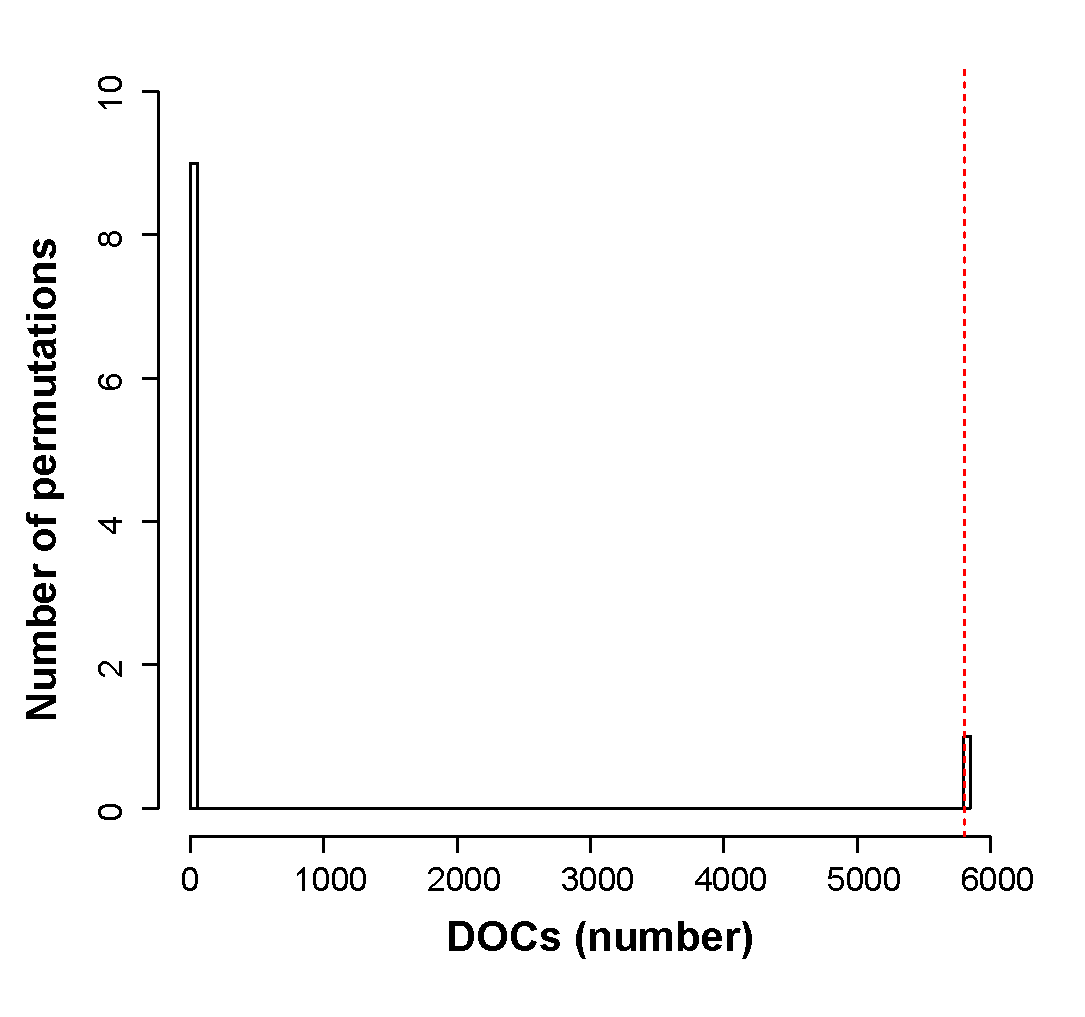
\includegraphics[width=\textwidth]{./Appendix/pdfs/Chapter5/ATAC_PsA_CD14_permutation_analysis}
\caption{}
\end{subfigure}
~
\begin{subfigure}[b]{0.45\textwidth}
\centering 
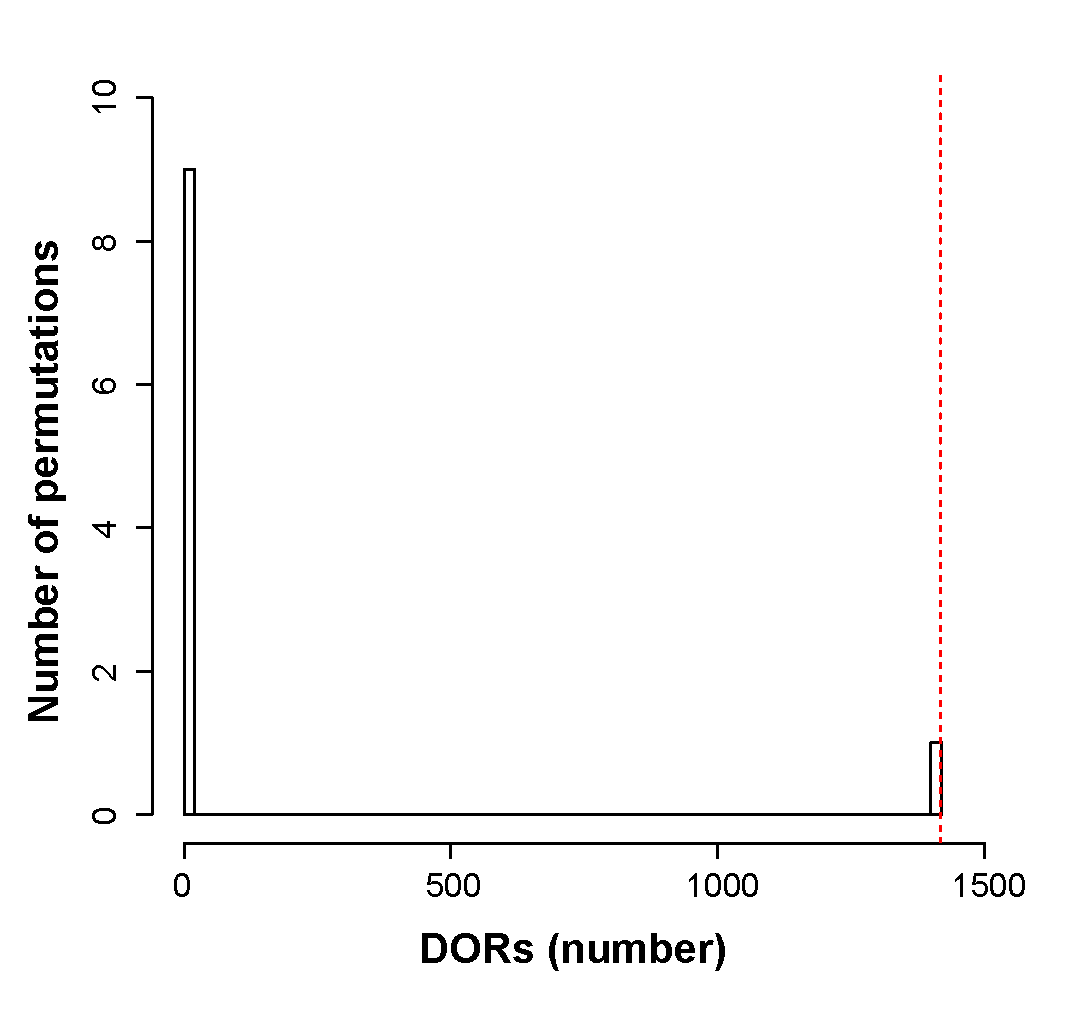
\includegraphics[width=\textwidth]{./Appendix/pdfs/Chapter5/ATAC_PsA_CD4_permutation_analysis}
\caption{}
\end{subfigure}
~
\begin{subfigure}[b]{0.45\textwidth} 
%the [b] prevents offset in subcaptions
\centering
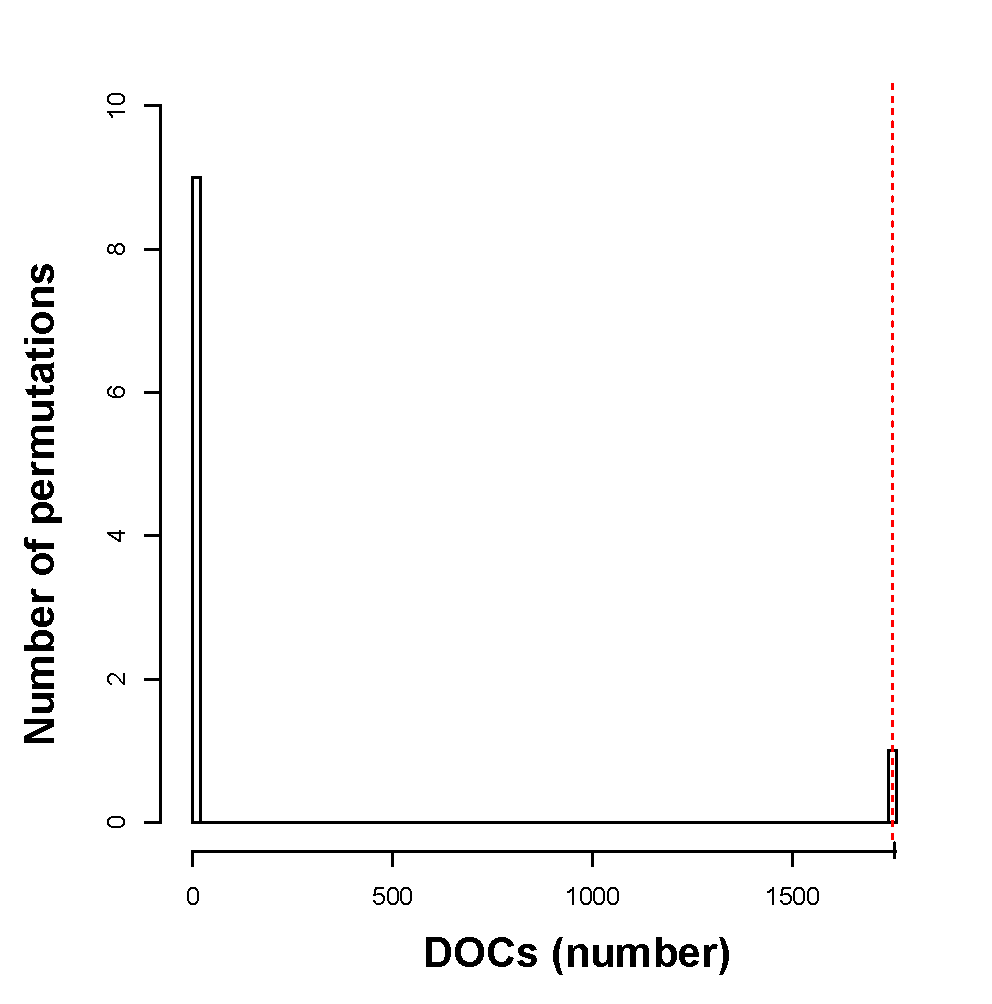
\includegraphics[width=\textwidth]{./Appendix/pdfs/Chapter5/ATAC_PsA_CD8_permutation_analysis}%
\caption{}
\end{subfigure}
\begin{subfigure}[b]{0.45\textwidth} 
%the [b] prevents offset in subcaptions
\centering
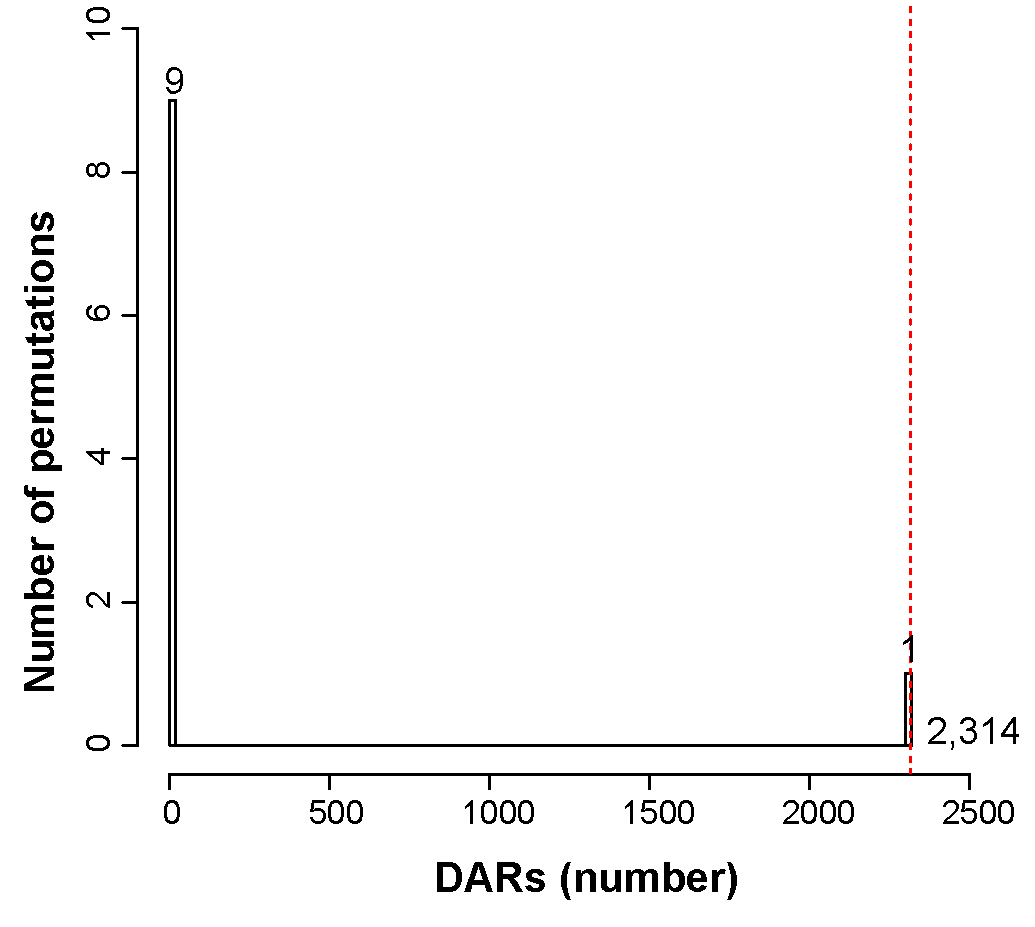
\includegraphics[width=\textwidth]{./Appendix/pdfs/Chapter5/ATAC_PsA_NK_permutation_analysis}%
\caption{}
\end{subfigure}
\caption[Permutation analysis SF vs PB in CD14$^+$ monocytes,CD4m$^+$,CD8m$^+$ and NK.]{\textbf{Permutation analysis SF vs PB in CD14$^+$ monocytes,CD4m$^+$,CD8m$^+$ and NK.} Sample labels were permuted within each cell type to achieve the ten unique possible combinations and differential analysis was performed. The number of significant DARs (FDR$<$0.01 and no abs(FC)$>$1.5) across all permutations in plotted for (A) CD14$^+$ monocytes, (B) mCD4$^+$, (C) mCD8$^+$ and (D) NK, demonstrating that the true observation (dashed red line) is significantly more than expected by chance (p-value$<$0.1, the lowest p-value for the maximum number of permutations that can be conducted with this sample size) in all four cell types.}
\label{figure:PsA_perm_analysis}
\end{figure}



\begin{figure}[htbp]
\centering
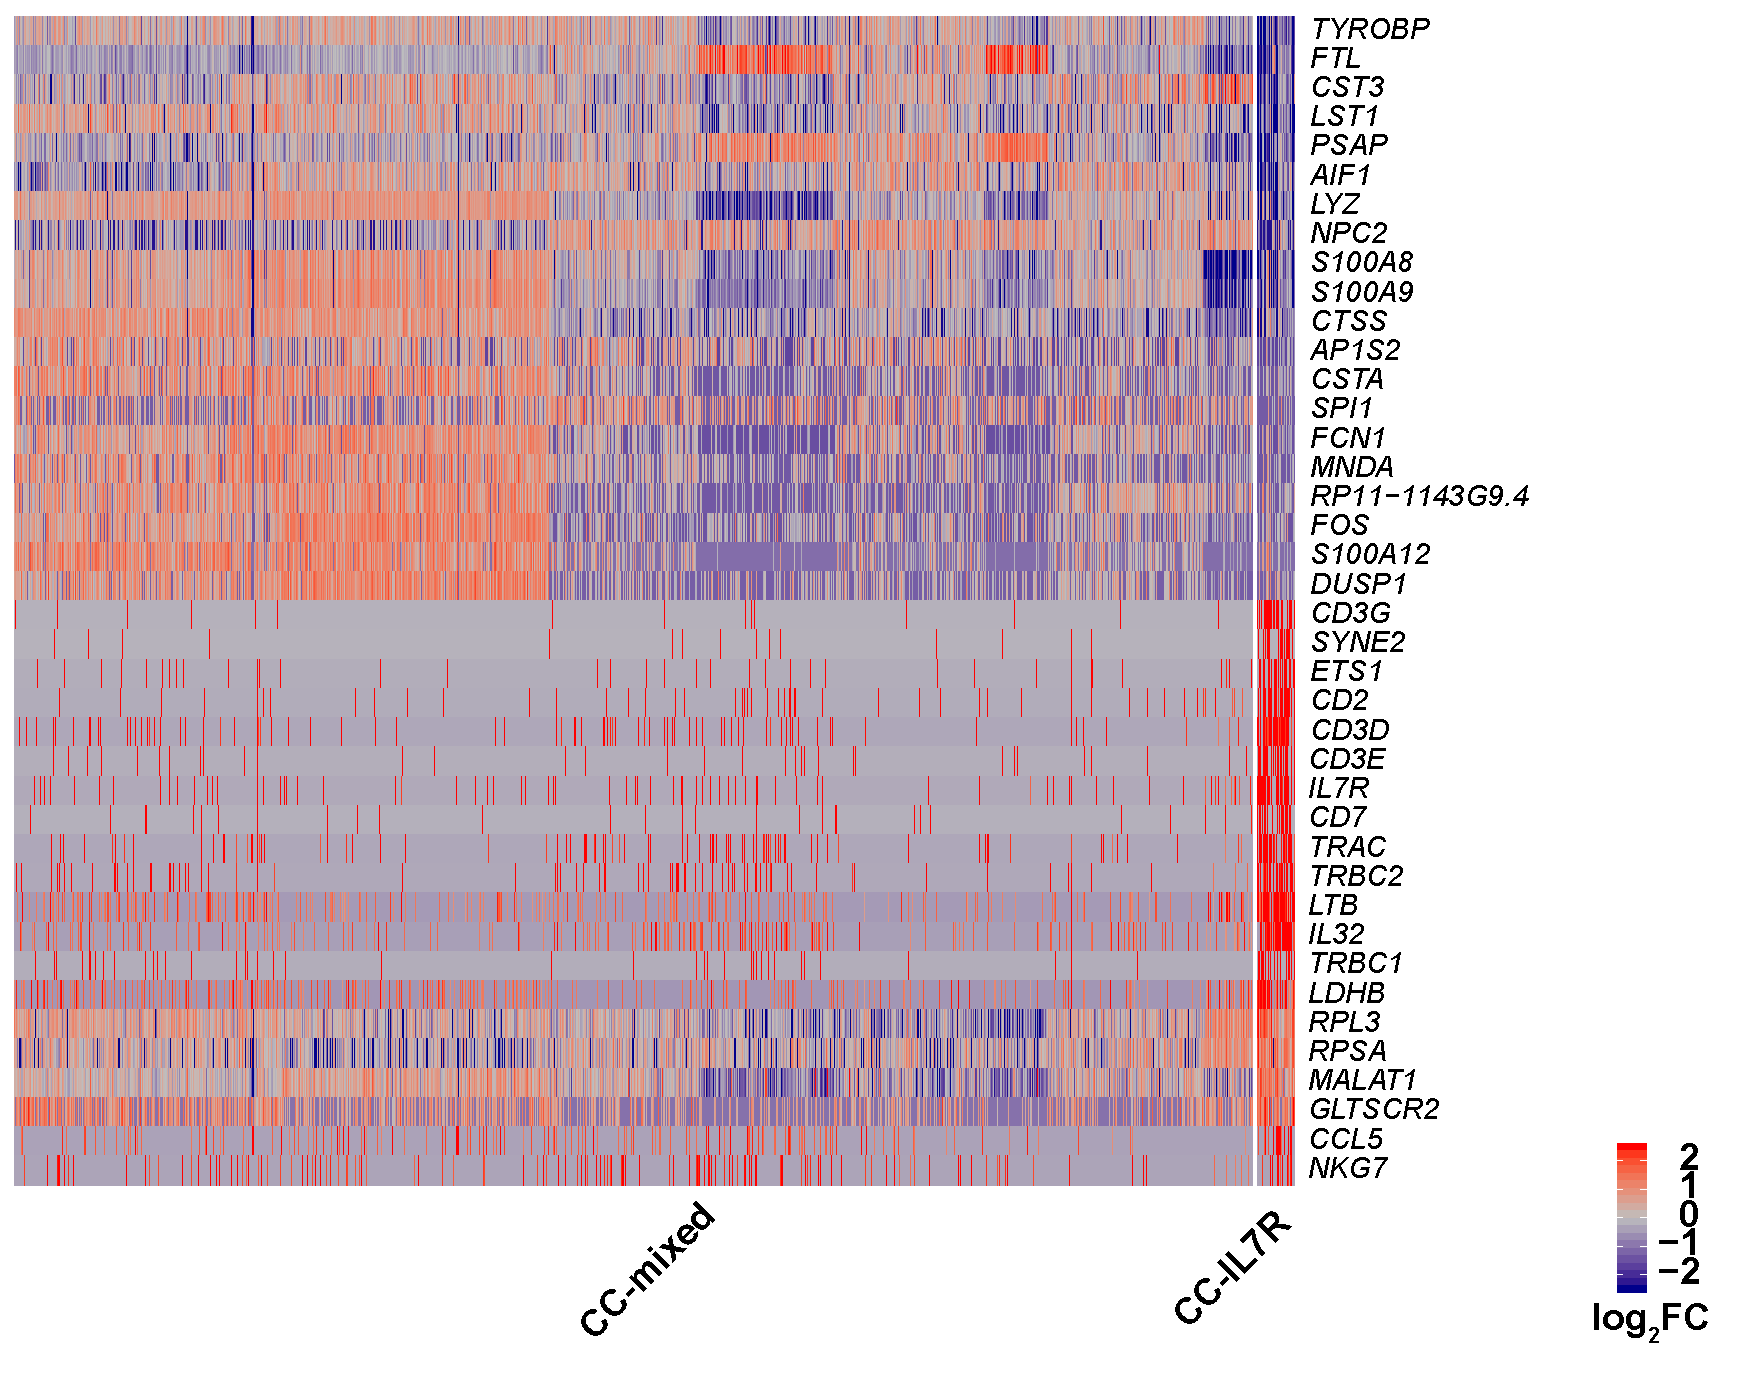
\includegraphics[width=0.6\textwidth]{./Appendix/pdfs/Chapter5/PSA_10X_heatmap_SF_PB_monocytes_clusters_mixed_and_IL7R}
\caption[Heatmap for the top 20 marker genes of the CC-mixed and CC-IL7R CD14$^+$ monocytes subpopulations.]{\textbf{Heatmap for the top 20 marker genes of the CC-mixed and CC-IL7R CD14$^+$ monocytes subpopulations.} Rows are the top 20 marker genes for each of the two subpopulations (total of 40 genes). The columns represent each of the cells members of the CC-mixed (left) or CC-IL7R (right) clusters. The colour scale represents the log$_2$FC in the expression of the marker gene in a particular cell of the cluster compared to the average expression of all the cells from the other cluster.}
\label{figure:PSA_scRNAseq_CC_mixed_and_IL7R_markers_heatmap}
\end{figure}

\bigskip
\begin{figure}[htbp]
\centering
\begin{subfigure}[b]{0.70\textwidth}
\centering 
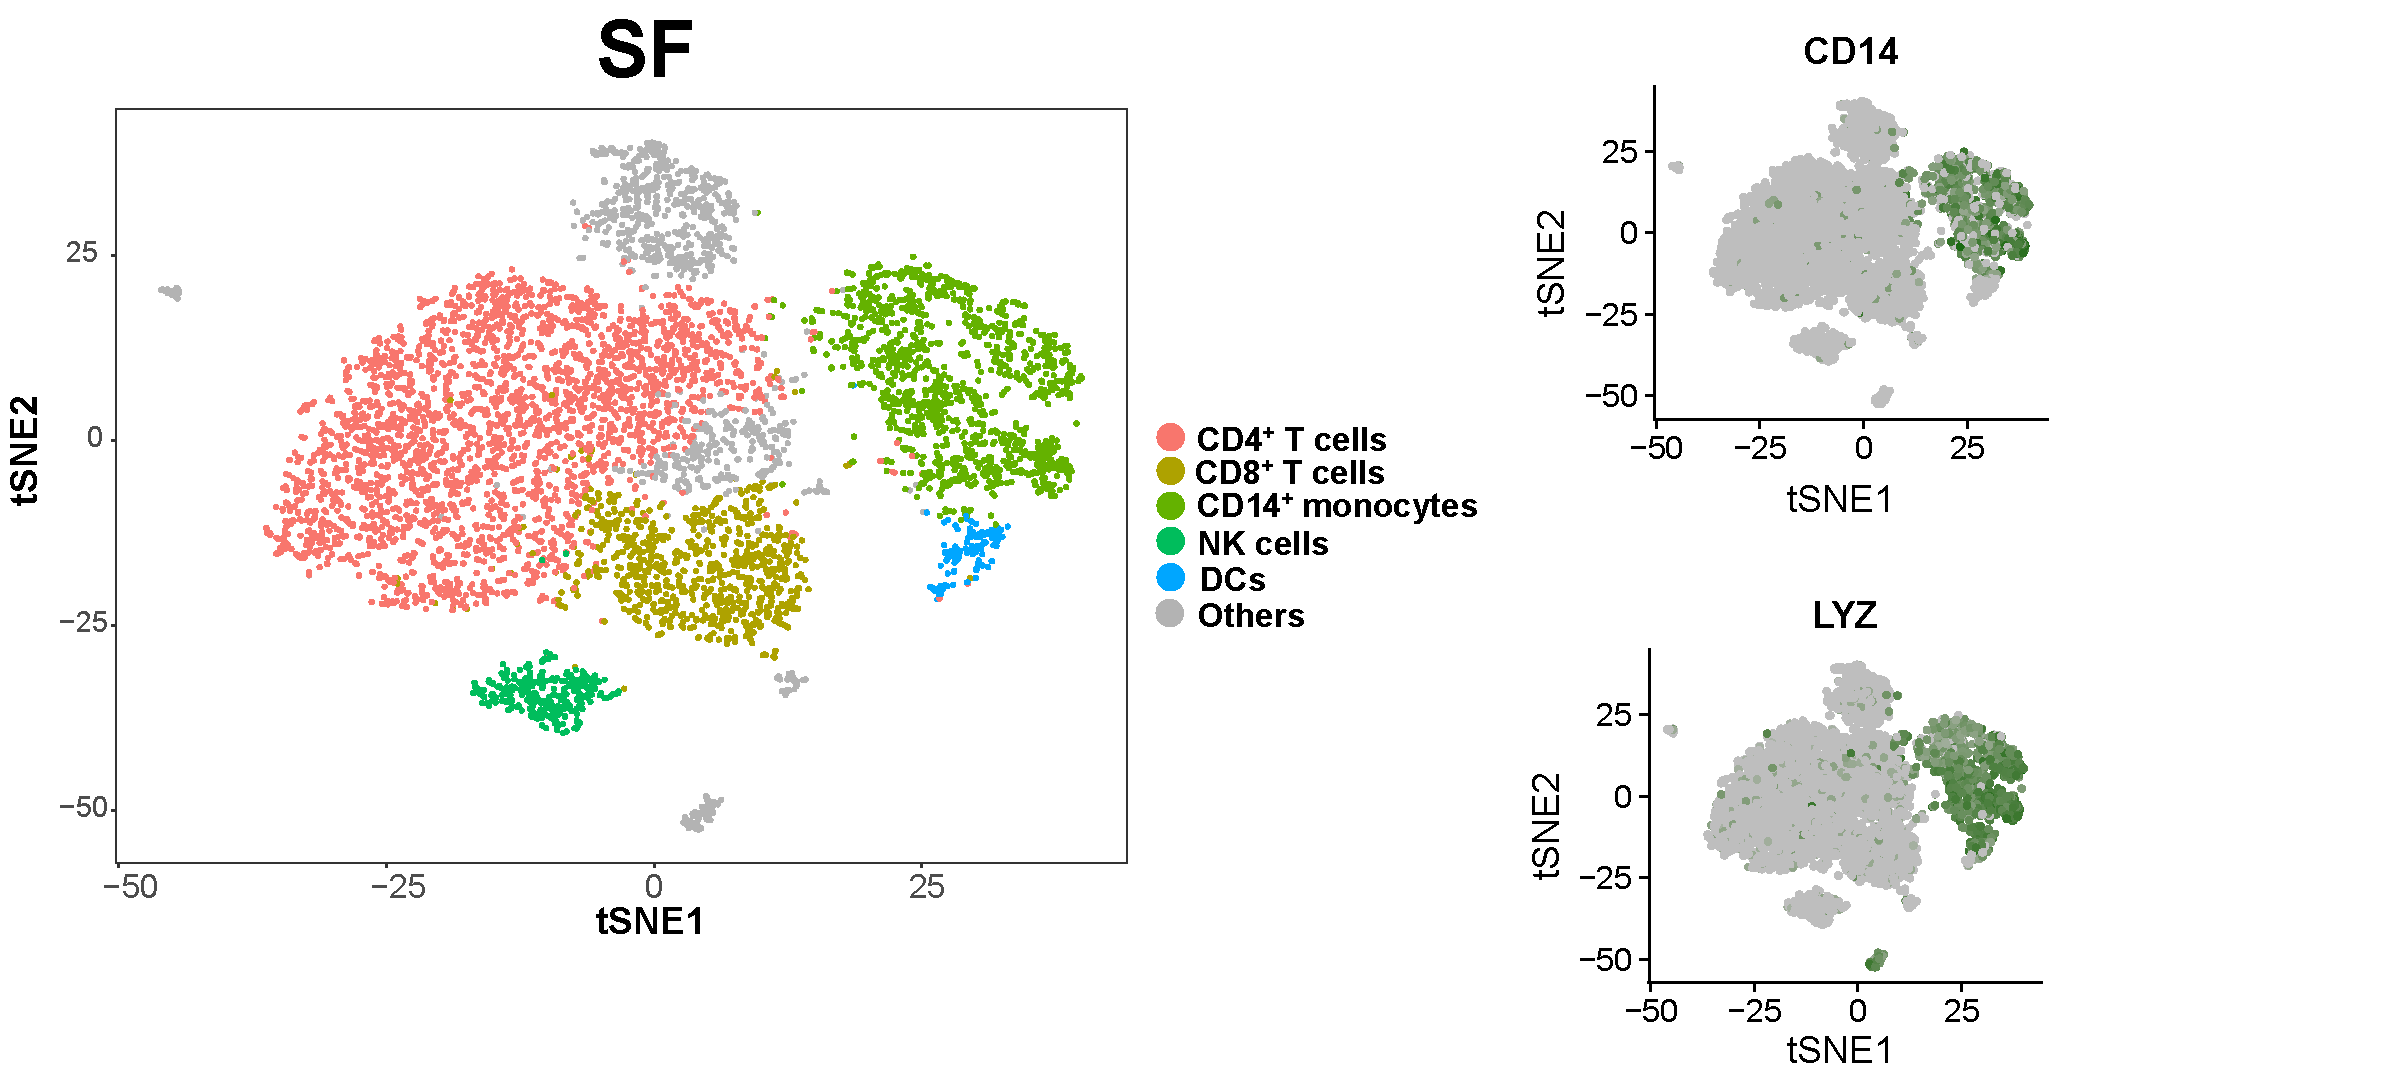
\includegraphics[width=\textwidth]{./Appendix/pdfs/Chapter5/PSA_SF_clusters_and_monocytes_markers}
\caption{}
\end{subfigure}
~
\begin{subfigure}[b]{0.70\textwidth} 
%the [b] prevents offset in subcaptions
\centering
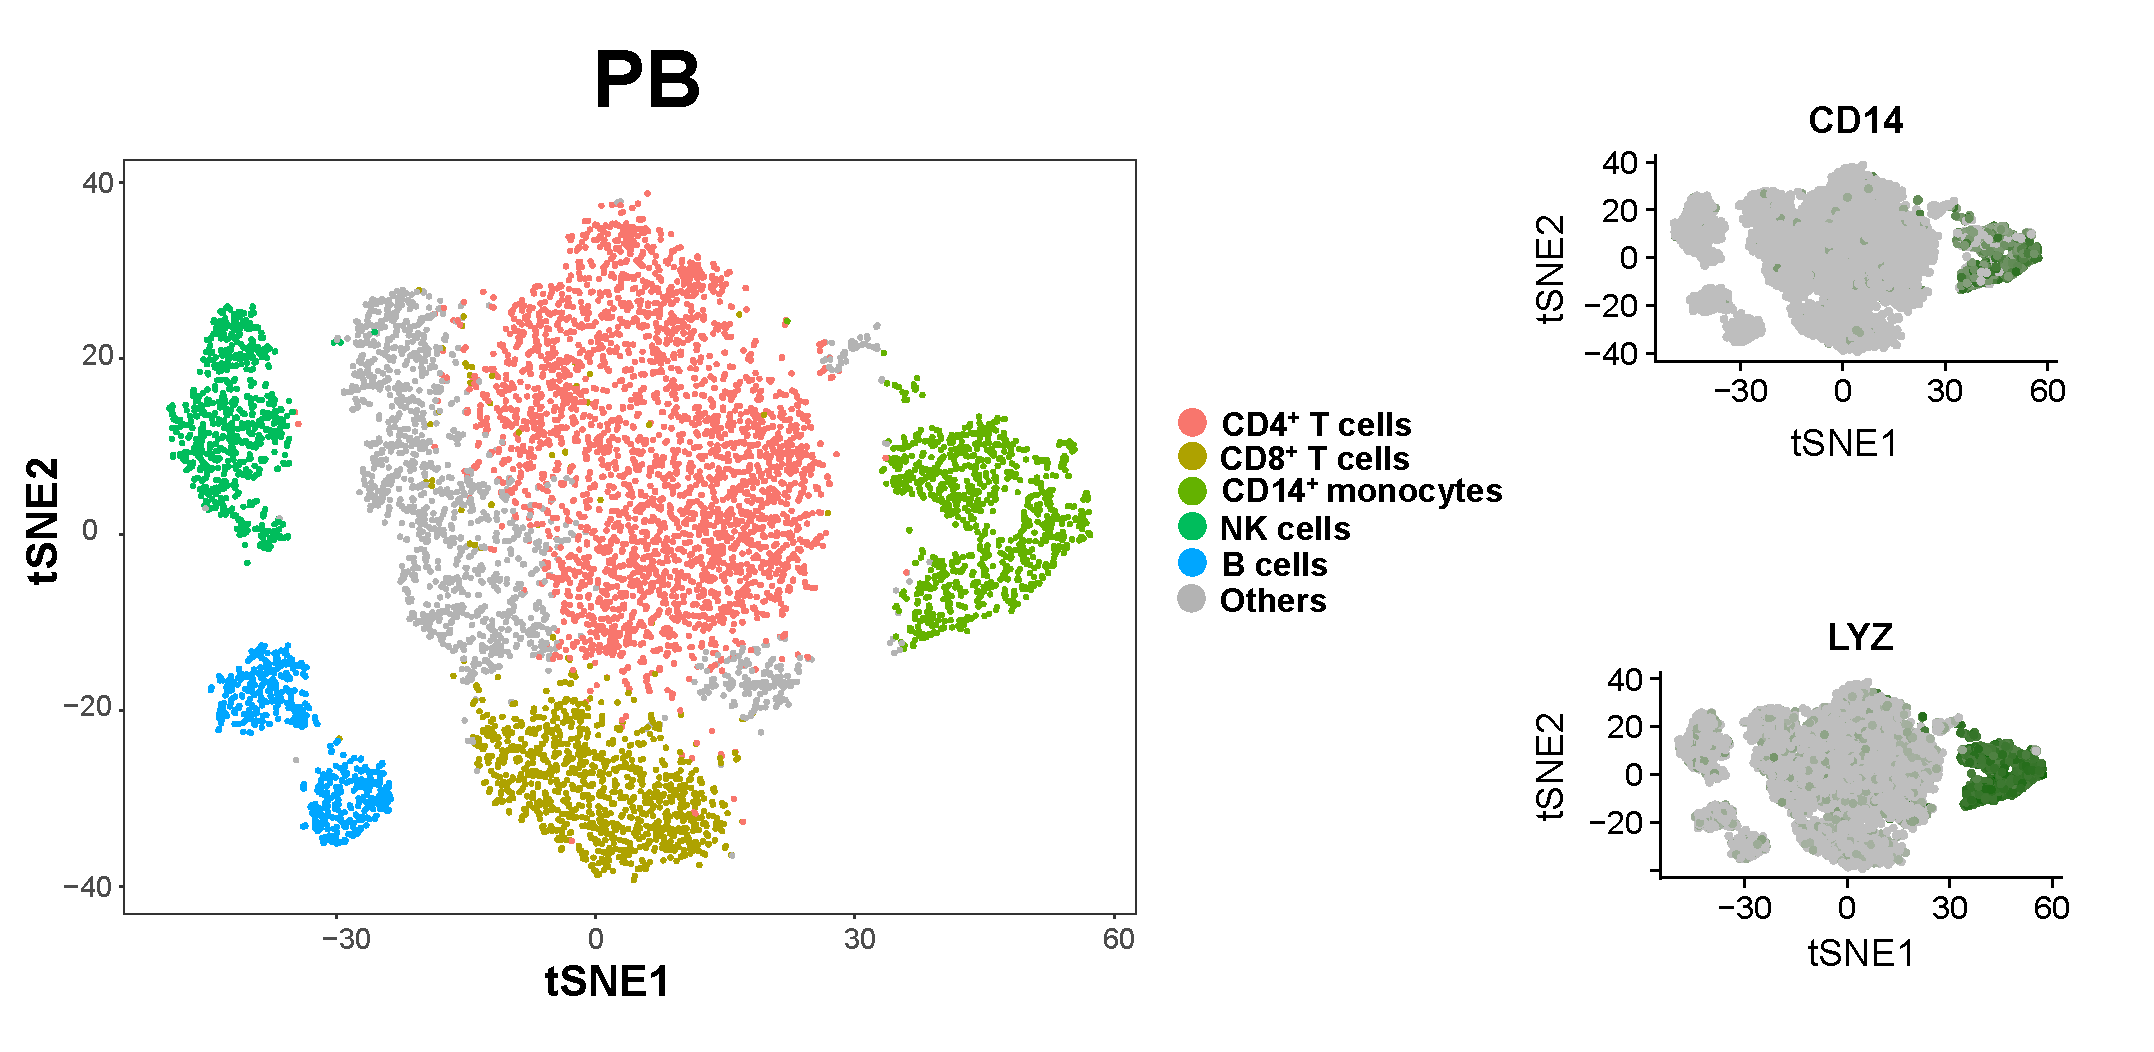
\includegraphics[width=\textwidth]{./Appendix/pdfs/Chapter5/PSA_PB_clusters_and_monocytes_markers}
\caption{}
\end{subfigure}
\caption[Identification of the CD14$^+$ monocytes populations from bulk SFMCs and PBMCs using scRNA-seq transcriptomes.]{\textbf{Identification of the CD14$^+$ monocytes populations from bulk SFMCs and PBMCs using scRNA-seq transcriptomes.} Visualisation using t-SNE dimensional reduction of the cell subpopulations identified in (A) SFMCs and (B) PBMCs and the overlay of CD14$^+$ monocytes characteristic markers (left hand side panel of (A) and (B))  for a representative PsA sample. Clustering performed using recommended resolution (res=0.6) allowed to identify CD4$^+$ (pink), CD8$^+$ (khaki), CD14$^+$ monocytes (green), NK (purple), DCs (blue), B cells (red) and others (grey). On the left hand side panel, expression for two characteristics CD14$^+$ monocytes markers (\textit{CD14} and \textit{LYZ}) used to subset this population (dark green dots) is overlaid on the t-SNE visual representation of all the cells in each of the tissues.}
\label{figure:PsA_scRNAseq_SF_an_PB_monocytes_identification_from_bulk}
\end{figure}




\begin{figure}[htbp]
\centering
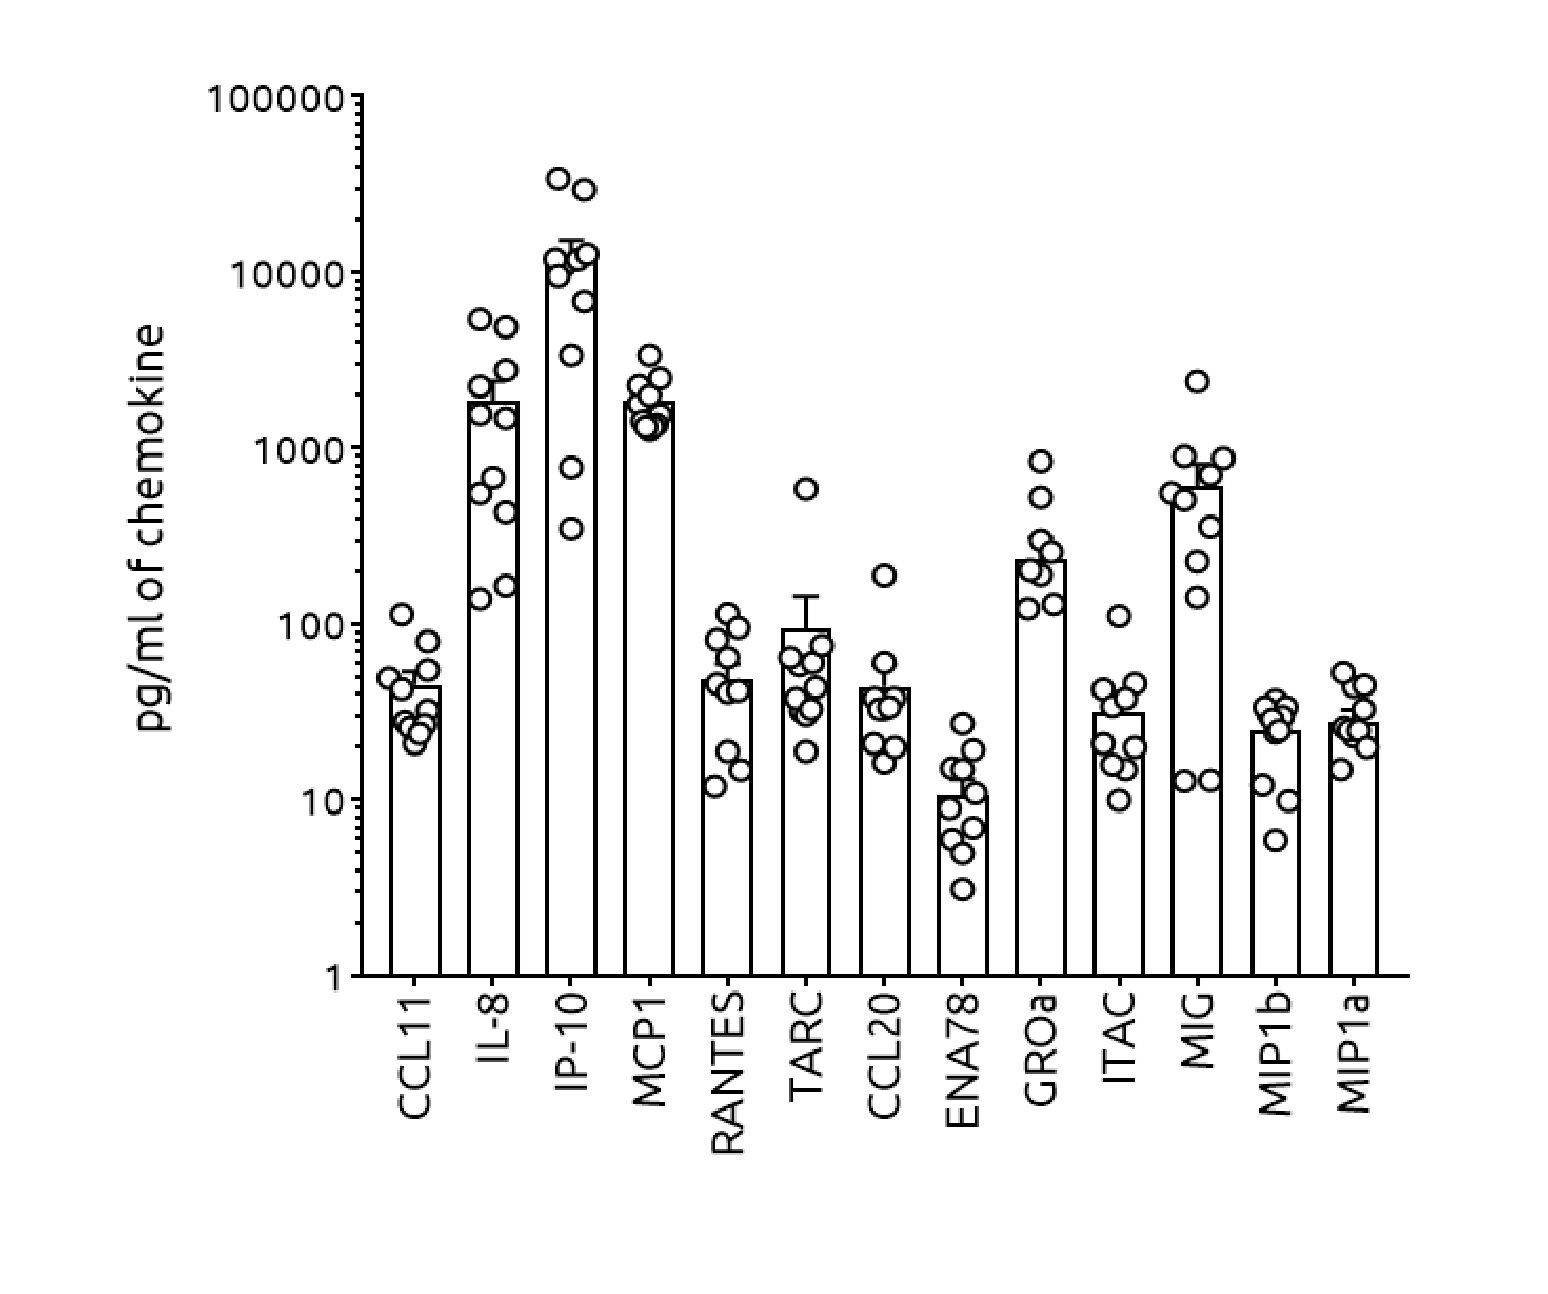
\includegraphics[width=0.5\textwidth]{./Appendix/pdfs/Chapter5/PSA_SF_elisa_cytokines_quantification}
\caption[Quantification of cytokine levels in SF from ten PsA patients.]{\textbf{Quantification of cytokine levels in SF from ten PsA patients.} Barplot graph illustrating pg/mL (x-axis) for a number of cytokines measured from SF of ten PsA patients by collaborators at University Basle using enzyme-linked immunosorbent assay (ELISA). Each circle represents a patients and error bars represent the standard deviation (SD) of the mean from all patients combined. Measurement for the same cytokines was performed in matched plasma from the same patients and all of them failed to be detected.}
\label{figure:ELISA_SF_PsA}
\end{figure}
